\chapter{Antecedentes}
\label{chap: cap3}

En esta sección se establecen referencias que sirven de modelo o ejemplos para este trabajo de investigación. Incluyen metodologías y tecnologías que anteceden al prototipo planteado, es decir, trabajos en los que se manejan parámetros y objetivos similares que sirven de guía para realizar comparaciones y tener ideas sobre cómo se solucionaron los problemas planteados.



\section{Antecedentes Metodológicos}

Desde 1980 hasta fines de 1990 los diseñadores se enfocaron en el diseño de software de la misma manera que lo habían hecho con el resto de los materiales. \vskip
Cuando se diseña para producir un objeto tangible, se necesita tener muy claro lo que se hace antes de iniciar la producción física, porque la producción es costosa, es costoso poner en marcha una fábrica para producir bienes físicos. \vskip En el ámbito del desarrollo de software, los diseñadores tuvieron que enfrentar nuevos retos, descubrir los nuevos medios y, a medida que lo hacían, aparecían nuevas especialidades, como el diseño de interacción o la arquitectura de información. Sin embargo, en esa época la práctica de los diseñadores apenas cambió. Todavía diseñaban los productos de manera tradicional, con mucho detalle y por adelantado, porque había un proceso de ``fabricación": había que hacer copias de los trabajo en discos flexibles y CDs y distribuirlas de la misma manera en la que se distribuyen los bienes físicos. Cometer errores en ese contexto se traducía en enormes costos de producción. \vskip

Internet cambió la lógica de distribución de software de una manera radical, la mayoría del software hoy en día se distribuye en línea y al desaparecer el proceso físico de fabricación se puede trabajar con ciclos de producción mucho más cortos.\vskip
Sin embargo el porcentaje de fracazos en los proyectos de software es notable, a continuación se realiza un análisis sobre este hecho:

\subsection{Análisis sobre fracazos y éxitos de los proyectos TI}
\textquote{\textit{En 1986, Alfred Spector, presidente de Transarc Corporation, fue coautor de un documento que compara la construcción de puentes con el desarrollo de software. La premisa: los puentes normalmente se construyen a tiempo, en presupuesto, y no se rompen. Por otro lado, el software nunca llega a tiempo o dentro del presupuesto y además, siempre se rompen}}  \citep{Mulder1995}, (sin embargo, la construcción de puentes no siempre tuvo un registro tan estelar. Muchos proyectos de construcción de puentes excedieron sus estimaciones, plazos de tiempo y algunos incluso se rompieron.\vskip
Una de las principales razones por las cuales los puentes se finalizan a tiempo, dentro del presupuesto y no se caen es por el detalle extremo del diseño. El diseño se cierra de antemano y el contratista tiene poca flexibilidad para cambiar las especificaciones. Sin embargo, en el entorno empresarial de rápido movimiento de la actualidad, un esquema con un diseño cerrado no admite cambios en las prácticas comerciales. Por lo tanto, es necesario el uso modelos más flexible. Esto podría ser y ha sido la razón fundamental para el fracaso de los desarrollos.

Pero hay otra diferencia entre las fallas del software y las fallas del puente, además de 3.000 años de experiencia. Cuando un puente se cae, se investiga y se escribe un informe sobre causa de la falla. Esto no es así en la industria del software donde las fallas muchas veces se ignoran. Como resultado, se siguen cometiendo los mismos errores una y otra vez.
En consecuencia, el foco en los proyectos de investigación de la agencia \textbf{The Standish Group}\footnote{\url{https://www.standishgroup.com/}} ha sido identificar:
\begin{itemize}
    \item El alcance de las fallas del proyecto de software.
    \item Los principales factores que hacen que los proyectos de software fallen.
    \item Los factores clave que pueden reducir las fallas del proyecto.
\end{itemize}


AGREGAR factores https://www.infoq.com/articles/standish-chaos-2015

El \textbf{Informe del Caos} en inglés \textit{Chaos Report} es publicado desde 1994 y cada dos años por ``Standish Group'', dando una visión sobre el fracaso o éxito de los proyectos en el sector de las TI, en inglés \textit{Information Technology} (IT). \textquote{\textit{Para el informe del 2015 se estudiaron 50000 proyectos en todo el mundo, desde pequeñas mejoras hasta implementaciones masivas de reingeniería de sistemas}} \citep{Hastie2015}. \vskip

Los proyectos en el informe se clasifican de la siguiente manera:
\begin{itemize}
    \item \textbf{Exitosos}: Son aquellos en los que no hay duda de que fueron un éxito.
    \item \textbf{Discutidos}: Son aquellos en los que hay dudas sobre si tuvieron éxito o fueron un fracaso
    \item \textbf{Fallidos}: Son aquellos en los que no hay duda de que fueron un fracaso
\end{itemize}

El éxito de estos proyectos se mide de acuerdo a tres variables:

\begin{itemize}
    \item \textbf{Acabado en plazos}.
    \item \textbf{Acabado en presupuesto}.
    \item Y \textbf{con resultados satisfactorios} (en el 2015 se elimina la categoría ``Acabado en alcance'' dada la necesaria variabilidad del mismo en el sector, recalculándose los cinco años anteriores con este criterio).
\end{itemize}

A continuación se pueden ver las cifras calculadas en el informe desde el 2011 al 2015.

%\begin{center}
% \begin{tabular}{ c | p{2cm} p{2cm} p{2cm} p{2cm} p{2cm} } 
%   \empty & 2011 & 2012 & 2013 & 2014 & 2015  \\ 
%   \hline
 %  Exitosos & 29\% & 27\% & 31\% & 28\% & 29\%  \\
 %  \hline
 %  Discutidos & 49\% & 56\% & 50\% & 55\% & 52\%   \\
%   \hline
 %  Fallidos & 22\% & 17\% & 19\% & 17\% & 19\% \\
%   \hline
  
%\end{tabular}
%\end{center}

\begin{figure}[h]
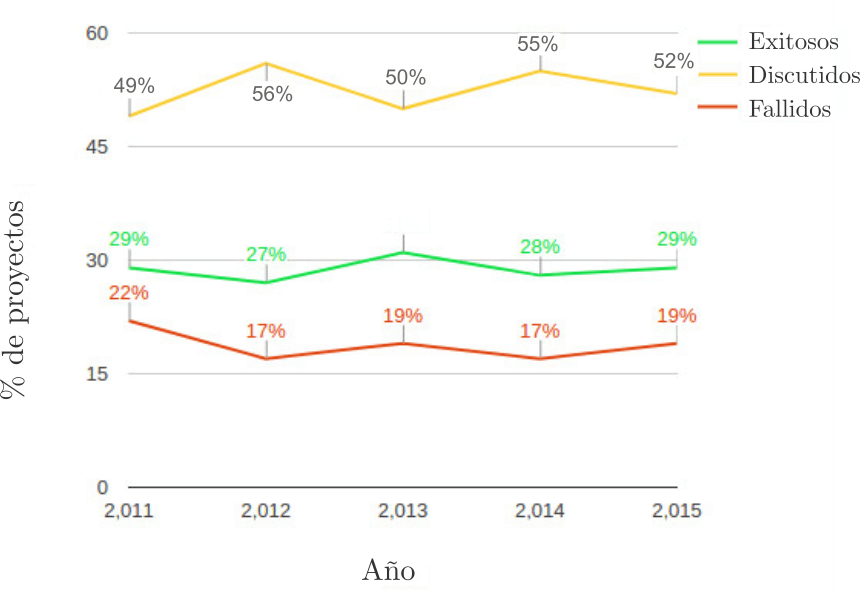
\includegraphics[width=11cm]{Img/Desarrollo/caos0.png}
\centering
\caption{\textbf{ \footnotesize{Proyectos, exitosos, discutidos y fallidos de 2011 hasta el 2015}}}
\label{fig:caos0}
\end{figure}

Lo primero que se destaca de esta comparativa es que del total de proyectos no hay ninguna tendencia en el éxito, se muestra oscilante sobre los mismos valores: el éxito entorno al 29\%, los discutidos entorno al 50\% y los fallidos entorno al 19\%. 

Hay otros factores para analizar que afectan al éxito o fracaso de los proyectos. Si se segmenta el informe por el tamaño de los proyectos como se puede apreciar en la figura \ref{fig:caos1} , el resultado es claro e incluso esperado.
Se muestran los proyectos exitosos desde 2011 a 2015 desde la perspectiva del tamaño. El dato es muy significativo y confirma que más del 62\% de los proyectos exitosos son pequeños. Está claro que los proyectos grandes son exponencialmente más complejos que los proyectos pequeños y los proyectos gigantes son prácticamente imposibles de controlar.

\begin{figure}[h]
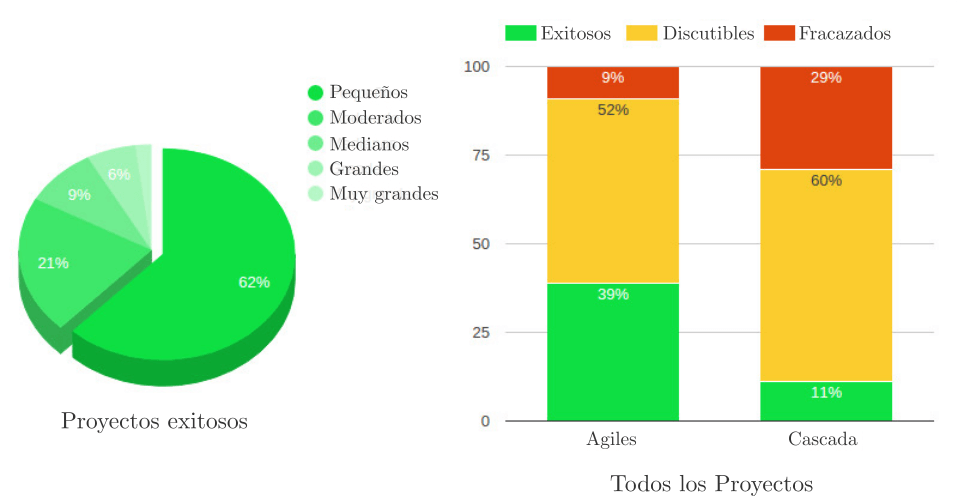
\includegraphics[width=15cm]{Img/Desarrollo/caos1.png}
\centering
\caption{\textbf{ \footnotesize{Éxito de los proyectos según su tamaño y métricas según la metodología.}}}
\label{fig:caos1}
\end{figure}

Otra información interesante que ofrece el Chaos Report es la comparativa del éxito de los proyectos en función de la metodología seguida para su desarrollo: \textbf{ágil vs cascada}.

\begin{figure}[h]
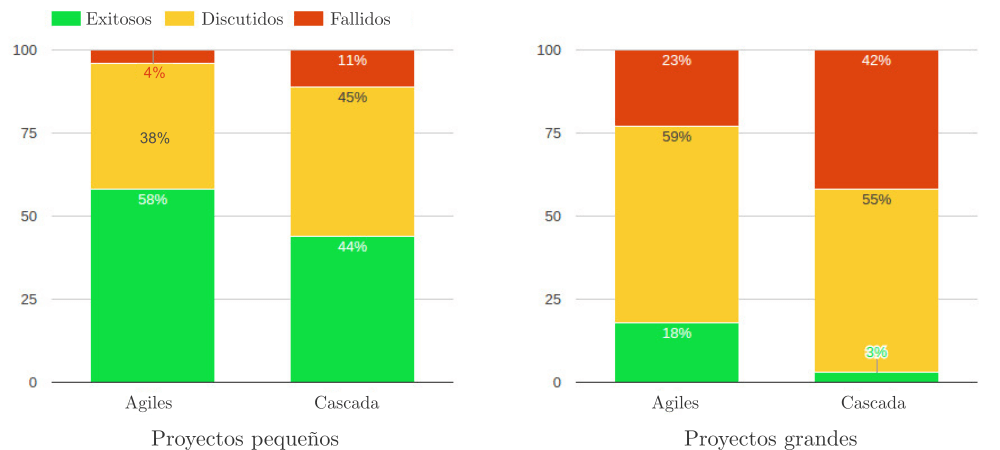
\includegraphics[width=15cm]{Img/Desarrollo/caos2.png}
\centering
\caption{\textbf{ \footnotesize{Métricas de los proyectos según la metodología.}}}
\label{fig:caos2}
\end{figure}

En los proyectos pequeños la diferencia no es tan grande pero es evidente. Los proyectos ágiles siguen siendo los más exitosos aunque por un margen menor. Ahora bien cuando el tamaño aumenta hacia proyectos grandes la diferencia se vuelve mucho más grande.

Al revisar los datos se evidencia que existen muchos más proyectos en cascada que ágiles y que el dato que se muestra es relativo debido a la naturaleza dinámica de los proyectos de soluciones digitales, es decir la muestra en ambos casos puede ser inexacta.
Aún así, por los datos presentados, los proyectos ágiles son mucho más éxitos que los no ágiles.\vskip
Con estos datos se puede verificar que la metodología en sí no es el único motivo para la mejora del éxito de los proyectos sino que, si se divide el problema en partes más manejables, más pequeñas y se trabaja progresivamente será más sencillo tener éxito.



%https://www.infoq.com/articles/standish-chaos-2015

%http://www.laboratorioti.com/2016/05/16/informe-del-caos-2015-chaos-report-2015-bien-mal-fueron-los-proyectos-ano-2015/
\clearpage

\clearpage
\subsection{Lean UX}
\label{section:pmv}
Los equipos de desarrollo de software en la actualidad utilizan técnicas como el desarrollo ágil, la integración continua y el despliegue continuo reduciendo drásticamente el tiempo para generar nuevas cambios en el software. Estos equipos realizan cambios en el código y suben los cambios a producción\footnote{Producción es la instancia del software cuando se encuentra a disposición de los usuarios finales.} con velocidad similar a la acción de guardar cualquier archivo en una computadora. Además, utilizan esos ciclos cortos como ventaja competitiva, producen nuevas versiones del software en tiempos acotados, lo que permite obtener retroalimentación del mercado e iterar incorporando lo que han aprendido y tal vez sin advertirlo aumentan las expectativas de los clientes que pueden obtener más calidad en menos tiempo. En este nuevo contexto, las prácticas de pensar todo al inicio de los procesos quedaron obsoletas. \vskip
\textbf{Lean User Experience} (Lean UX) se puede traducir como \textbf{Experiencia de Usuario limpia o sin desperdicios}. Jeff Gothelf y Josh Seiden lo describen como \textquote{\textit{una nueva etapa evolutiva en el diseño de productos. Esta metodología utiliza las mejores herramientas de las que disponemos y las combina de forma diferente para adecuarlas a esta nueva realidad}} \citep{Gothelf2013}.


Lean UX es profundamente colaborativo y multifuncional, en gran medida porque:
\begin{itemize}

    \item Logra que los diseñadores no están aislados del resto del equipo de trabajo.
    \item Permite implementar técnicas para construir una comprensión compartida del proyecto. 
    \item Logra un clima propicio para la retroalimentación con los usuarios finales y  replantea las conversaciones de diseño en términos objetivos, se pueden obtener métricas sobre las funcionalidades, analizar y ajustar.
    \item Cambia la forma en que se comunica el diseño del producto: En lugar de hablar de funciones y documentos, se puede hablar de lo que efectivamente funciona y de lo que no.

\end{itemize}

\textquote{\textit{Lean UX es tres cosas. Es fácil ver que se trata, en primer lugar, de \textbf{un cambio de procesos para los diseñadores}. Pero es más que eso. También es \textbf{una nueva mentalidad que cambia la manera en la que nos enfrentamos a nuestro trabajo} . Y también \textbf{una nueva manera de pensar en la gestión de software}}} \citep{Gothelf2013}. 

\vspace{5mm}

Los \textbf{3 pilares principales de Lean UX} son:
\begin{enumerate}
    \item \textbf{Design Thinking o Pensamiento de Diseño} \vskip
    Tim Brown describió el \textbf{design thinking} como \textquote{\textit{innovación que se alimenta de […] la observación directa de lo que la gente quiere y necesita en sus vidas y lo que les gusta o disgusta de cómo se hacen los productos, cómo se empaquetan, cómo se ponen en el mercado, cómo se venden y cómo se les presta ayuda […]. Se trata de una disciplina que, utilizando la sensibilidad y los métodos de los diseñadores, satisface las necesidades del público con aquello que resulta tecnológicamente posible y que, gracias a una estrategia de negocio viable, puede convertirse en valor para los clientes y en oportunidades en el mercado}} \citep{Brown2009}. \vskip
    Lean UX considera importante el design thinking porque esta manera de concebir el diseño defiende una posición concreta para todos los aspectos del negocio que deban abordarse con él. Además, permite a los diseñadores superar los límites habituales que se les imponen en los proyectos. Por otra parte, anima a los no diseñadores a utilizar los métodos propios del diseño para resolver los problemas de sus respectivas disciplinas. El design thinking es un pilar básico de esta metodología, una manera de trabajar que alienta la colaboración en el equipo, independientemente del rol que cada uno desempeñe, y que considera el producto desde una perspectiva abarcadora.

    \item \textbf{Metodologías de desarrollo ágil de software}.\vskip
    Los desarrolladores de software han usado durante mucho tiempo las metodologías de desarrollo ágil para reducir el ciclo de vida de sus productos y aportar de forma constante valor a sus clientes. No obstante, estas metodologías muchas veces constituyen un reto para los diseñadores.

     Aplican los cuatro principios básicos del \textbf{Desarrollo Ágil} al diseño de productos.
        
        \begin{enumerate}
        \item
        \textbf{Los individuos y las interacciones son más importantes que los procesos y las herramientas}\vskip
        Para generar rápidamente las mejores soluciones, es necesario implicar al todo el equipo. El intercambio de ideas deberá ser libre y frecuente. La conversación fluida entre colegas deberá primar por encima de las restricciones propias de las herramientas, ya sea en los procesos o en la producción.
        \item
        \textbf{El software funcional es más importante que la documentación exhaustiva}\vskip
        Se pueden encontrar múltiples soluciones para todos los problemas de negocio y todos los miembros del equipo podrán tener una opinión diferente de cuál es la mejor. El reto está en averiguar cuál de ellas es la que tiene más posibilidades. Por eso, cuanto antes se cuente con un software que funcione, antes se puede encontrar la solución que mejor se adapte a los requerimientos.
        \item
        \textbf{La colaboración con los clientes es más importante que la negociación de contratos con ellos}\vskip
        Si el equipo colabora con los usuarios/clientes, hay un entendimiento común sobre los problemas y las posibles soluciones. Cualquier decisión que se adopte después se tomará por consenso, lo que se traduce en iteraciones más rápidas y una verdadera implicación de todos los actores con la ventaja de trabajar siempre con soluciones validadas. Además, como todos los miembros del equipo participan en la toma de decisiones, no se requieren tantas entregas de documentación por escrito.
        \item
        \textbf{La respuesta a los cambios es más importante que la planificación}\vskip
        Lean UX asume que los diseñadores del producto inicial no encontrarán la solución a la primera, por lo que el objetivo consiste en averiguar qué han hecho mal lo antes posible. Una vez que se descubra lo que funciona y lo que no, se pueden ajustar las propuestas y volver a probarlas. Así, la retroalimentación mantendrá ágil al equipo, dirigiendo la solución siempre en la dirección correcta.
        \end{enumerate}

\item \textbf{Método Lean Startup}\vskip 
Lean Startup\footnote{\url{http://theleanstartup.com/}} utiliza un ciclo de feedback denominado \textbf{``crear-medir-aprender''} que minimiza el riesgo de los proyectos y que consigue que el equipo pueda desarrollar software y aprender de él en muy poco tiempo. Con este método, los equipos desarrollan lo antes posible los denominados \textbf{Productos Mínimos Viables} en inglés \textit{Minimum Viable Products} (MVP)\footnote{El producto viable mínimo MVP es un producto con suficientes características para satisfacer a los clientes iniciales, y proporcionar retroalimentación para el desarrollo futuro} para comenzar cuanto antes el proceso de aprendizaje. Tal y como indica Eric Ries: \textquote{\textit{\textbf{Lean Startup} aboga desde el principio por la creación de prototipos rápidos para comprobar, por un lado, que las suposiciones que hemos hecho sobre el mercado son correctas y, por otro, para conseguir feedback de los clientes y así poder mejorar el software mucho más rápido que las prácticas tradicionales de ingeniería de software […] Al aumentar la frecuencia de contacto con clientes reales, se reduce el despilfarro y se prueban lo antes posible las ideas del equipo, evitando así las suposiciones incorrectas sobre el mercado}} \citep{Gothelf2013}. Lean UX, por su parte, consiste en la aplicación directa de esta filosofía al diseño de productos. En Lean UX, cada diseño es una solución propuesta para el problema, una hipótesis. El objetivo consiste en validar esa solución de una manera eficiente, utilizando para ello el feedback de los clientes/usuarios. \vskip
\vspace{5mm}
El proceso es el siguiente: 
    \begin{itemize}
    \item En primer lugar, se crea el MVP, es decir, \textbf{el desarrollo más pequeño que pueda construirse para probar cada hipótesis}. Los MVP no tienen por qué estar hechos solo de código de programación, también pueden ser aproximaciones, verbales o escritas, a la experiencia de usuario final. 
    \item A continuación, se muestra el MVP a los clientes/usuarios.
    \item Después, se utiliza lo aprendido de ellos para hacer modificaciones.
    \item Y entonces se itera, se comienza todo el proceso de nuevo. 
    \end{itemize} 
    
En la figura \ref{fig:leanux} se puede apreciar el proceso de este enfoque.
Lo que Lean UX hace en realidad es sacar a la luz más rápido la verdadera naturaleza de los productos. Para ello, elige un camino colaborativo y multifuncional, un camino que otorga más importancia a la creación de un entendimiento común de la experiencia de usuario que se está diseñando que a la creación y entrega de documentación.

\end{enumerate}


\begin{figure}[h]
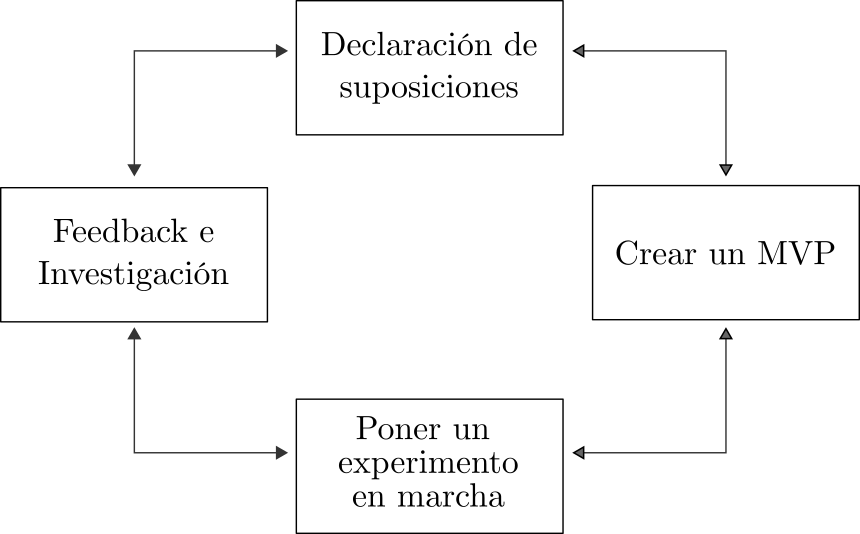
\includegraphics[width=10cm]{Img/Desarrollo/desarrollo0.png}
\centering
\caption{\textbf{ \footnotesize{Proceso del enfoque LEAN UX. }}}
\end{figure}
\label{fig:leanux}

En resúmen, Lean UX funciona como una práctica para entender rápidamente la función de un producto. Para ello elije un camino colaborativo y multidisciplinario; reduce el énfasis por la documentación exhaustiva y aumenta el enfoque en la construcción de un entendimiento compartido del producto que está siendo diseñado. Como consecuencia de usar este enfoque se obtiene: un equipo que trabaja de forma colaborativa, iterativamente, reduciendo al mínimo los documentos entregables, enfocándose en el software funcional y en la retroalimentación con el usuario final.

\subsubsection{Principios de LEAN UX}
Lean UX contiene en su núcleo un juego de principios clave, que abarcan el proceso de diseño, la colaboración, la gestión, etc., para que los equipos puedan sacarle el máximo provecho al enfoque propio de la metodología. Se consigue con ellos que los equipos se encaminen en la dirección correcta y sean especialmente útiles para implementar los procesos de Lean UX. Los procesos, sin duda se deben ajustar a cada proyecto, por ende los principios se utilizan como guía y no de forma obligatoria. \vskip

A continuación se explican los principios:
\begin{itemize}
    \item \textbf{Principio: Equipos multifuncionales}\vskip 
    ¿De qué se trata? Los equipos multifuncionales deben incluir todas las disciplinas que intervienen en la creación del producto. La ingeniería del software, la gestión del producto, el diseño de interacciones, el diseño gráfico, la estrategia de contenidos y el control de calidad (QA), todas deben contar con representantes en ellos. Lean UX necesita que todos los que se dedican a estos campos colaboren intensamente, por lo que la implicación del equipo debe ser continua, desde el primer día del proyecto hasta el final.\vskip
    ¿Por qué hacerlo? Estos equipos, diversos en su constitución, evitan el desarrollo en cascada, con su proceso rígido de entregas de documentación. En su lugar, todos los campos aportan conocimiento mucho antes al proceso. Como la metodología promueve, además, que los miembros de los diferentes ámbitos hablen entre ellos, la eficacia del equipo aumenta.
    
\item \textbf{Principio: Pequeños, dedicados, coubicados }\vskip 
    ¿De qué se trata? Es necesario limitar el tamaño de los equipos, no deben ser mayores de diez personas, dedicados exclusivamente al proyecto y trabajando en el mismo lugar. \vskip
    ¿Por qué hacerlo? El beneficio de los equipos pequeños se resume en tres palabras: comunicación, concentración y camaradería. Así se comunica de forma sencilla sobre el estado del proyecto, de los cambios y del nuevo conocimiento que surja. La dedicación en exclusiva, por otra parte, hace que todos los miembros estén centrados en las mismas prioridades. Y además, trabajar en el mismo lugar hace las relaciones entre colegas sean más estrechas.
    
    \item \textbf{Principio: Equipos centrados en los problemas}\vskip
    ¿De qué se trata? Un equipo centrado en los problemas es un grupo que sabe que debe resolver el problema asignado y no limitarse a implementar un grupo de funciones. Este principio es una extensión lógica del anterior, que afirmaba que el progreso del proyecto dependía de los resultados.\vskip
    ¿Por qué hacerlo? Si se asignan problemas completos a un equipo se demuestra más confianza en las personas que lo conforman. Además, así se les permite llegar a sus propias soluciones, con lo que se consigue aumentar la sensación de pertenencia en el proyecto.
    
    \item \textbf{Principio: Eliminación del desperdicio}\vskip
    ¿De qué se trata? Una de los prácticas principales de \textbf{Lean manufacturing}\footnote{Lean manufacturing es un modelo de gestión enfocado en la creación de flujo para poder entregar el máximo valor a los clientes. Para ello, utiliza la mínima cantidad de recursos, es decir, los necesarios} es la eliminación de todo lo que no contribuya a conseguir el objetivo final. En Lean UX, este objetivo final es la producción de mejores resultados, por lo que todo lo que no ayude a conseguirlos se considera despilfarro y debe eliminarse del proceso de trabajo del equipo.\vskip
    ¿Por qué hacerlo? Los recursos del equipo son limitados, por lo que cuanto más desperdicio se elimine, más rápido podrán producir los miembros del equipo. En realidad, lo que los equipos necesitan es ser efectivos y trabajar en los retos adecuados, con la atención en donde se debe.
    
    \item \textbf{Principio: Lotes pequeños}\vskip
    ¿De qué se trata? Otra idea fundamental de Lean manufacturing es la utilización de lotes pequeños. En ese modelo, esta noción se usa para indicar que no se deben tener muchos productos en stock y que la calidad de producción debía ser alta. Adaptado a Lean UX, su significado es que el equipo solo debe crear los diseños necesarios para avanzar, evitando crear un gran stock de ideas de diseño sin probar ni implementar. \vskip
    ¿Por qué hacerlo? El diseño en grandes lotes resta eficiencia al equipo, ya que, para poder realizar grandes entregas de diseño, se insume mucho tiempo. En ese tiempo no se puede aprender si las ideas funcionan e, inevitablemente, algunos de los miembros tendrán que estar desocupados, aparte de generar recursos de diseño inútiles. Es decir, se trata de una estrategia con un despilfarro que no maximiza el potencial de aprendizaje del equipo.
    
    \item \textbf{Principio: Descubrimiento continuo }\vskip
    ¿De qué se trata? El descubrimiento continuo consiste en comprometer a los usuarios con el proceso de diseño y desarrollo, mediante actividades programadas con ellos en intervalos regulares, en las que se aplican métodos cualitativos y cuantitativos. El objetivo es entender lo que los usuarios hacen con productos y por qué lo hacen. La investigación con ellos debe realizarse de forma frecuente y regular y debe implicar al todo el equipo.\vskip
    ¿Por qué hacerlo? Las conversaciones regulares con los usuarios ofrecen oportunidades de validar nuevas ideas sobre el producto. Por otra parte, al incluir al equipo completo en el ciclo de desarrollo, estos desarrollarán empatía por los usuarios y por los problemas a los que tienen que enfrentarse. Además, como todos los miembros aprenden juntos en las reuniones, no será necesario generar demasiada documentación ni explicar lo sucedido en otras reuniones internas.
    
    \item \textbf{Principio: GOOB: La nueva centralidad del usuario}\vskip
    ¿De qué se trata? Se utiliza el acrónimo \textbf{``Salir del edificio''} en inglés \textit{Getting Out Of the Building} (GOOB). Significa que los debates sobre las necesidades de los usuarios no tienen por qué cerrarse en el mismo lugar en el que se desarrollan, es decir, en la oficina. Las respuestas, más bien, están en el mercado, fuera de ella. Después de mucho tiempo abogando por la investigación del comportamiento de los usuarios, la comunidad de experiencia de usuarios (UX) tiene un aliado en Steve Blank, que proviene del mundo de los negocios. Su consejo: \textquote{\textit{ofrezcamos la posibilidad a los clientes potenciales de dar su opinión sobre nuestras ideas mucho antes de lo que lo han hecho en el pasado. Mucho antes. Démosles un baño de realidad mientras aún están en su infancia. Es mucho mejor averiguar que nuestras ideas han errado el tiro antes de dedicar tiempo y recursos a construir un producto que nadie quiere}} \citep{Gothelf2013}.\vskip
    ¿Por qué hacerlo? En los últimos tiempos, el éxito o el fracaso de los productos no dependen de las decisiones del equipo de desarrollo, sino de los usuarios. Son ellos los que tendrán que utilizar los producto. Cuanto antes se los haga participar, antes se aprende si las ideas están listas para pasar a la fase de desarrollo.

    \item \textbf{Principio: Entendimiento común}\vskip 
    ¿De qué se trata? El entendimiento común es el conocimiento colectivo del equipo. Se construye poco a poco a medida que ese equipo trabaja de forma conjunta y consiste en una comprensión profunda del espacio, del producto y de los clientes.\vskip 
    ¿Por qué hacerlo? Este tipo de conocimiento es la moneda de cambio de Lean UX. Cuanto más sepa el equipo, como colectivo, de lo que está haciendo y de por qué lo está haciendo, menos dependerá de informes de segunda mano y de documentos detallados para continuar con su trabajo.
    
    \item \textbf{Principio: Antimodelos: estrellas, gurús y ninjas }\vskip 
    ¿De qué se trata? Lean UX aboga por una mentalidad de equipo. Las estrellas, los gurús, los ninjas y, en general, rompen la cohesión del equipo y reducen la colaboración.\vskip ¿Por qué hacerlo? Las estrellas no comparten las ideas ni la atención de los demás. Si se cuenta con individuos de este tipo en los equipos, con grandes egos y determinados a brillar por encima de todos, se rompe la colaboración del grupo. Si eso sucede no se cuenta con un entorno en el que se pueda construir un entendimiento común, necesario para avanzar de forma efectiva.
    
    \item \textbf{Principio: Exteriorización del trabajo}\vskip
    ¿De qué se trata? Con exteriorización me refiero a exponer el trabajo de forma pública, más allá de las computadoras. Los equipos pueden utilizar pizarras, tableros de cartón, paredes repletas de artefactos, salidas impresas, notas adhesivas, lo que sea que hayan utilizado para reflejar sus ideas, para poder mostrar el trabajo a compañeros, colegas y clientes.\vskip 
    ¿Por qué hacerlo? La exteriorización somete las ideas a escrutinio público y así todos los miembros del equipo pueden ver dónde se encuentran como grupo. De esta manera se crea un flujo de información que circula entre todos los miembros, información que está en el ambiente y que inspira nuevas ideas, construidas sobre las que se han compartido. Además, esta forma de trabajar hace participar a todos los miembros del equipo, incluso las personas tímidas, ya que las notas adhesivas, se tratan por igual.

    \item \textbf{Principio: Aprendizaje en lugar de crecimiento}\vskip
    ¿De qué se trata? Es complicado concebir una buena idea y hacerla crecer al mismo tiempo. Son actividades contradictorias. Lean UX apuesta por que, en primer lugar, se concentre en el aprendizaje y luego en su crecimiento.\vskip 
    ¿Por qué hacerlo? Escalar una idea que no se ha probado es arriesgado. Podría funcionar o podría no hacerlo. Si no lo hace y la idea se sube a producción para todos los usuario, en lugar de para unos cuantos con los que probar, el equipo habrá perdido tiempo y recursos valiosos en hacerlo. Al asegurarse de que una idea funciona antes de hacerla crecer, se reduce el riesgo que conllevan los grandes despliegues de funciones.
    
    \item \textbf{Principio: Hacer en lugar de analizar}\vskip
    ¿De qué se trata? Lean UX valora la acción por encima del análisis. Hay más valor en crear la primera versión de una idea que en emplear medio día debatiendo sus méritos en una sala de reuniones. ¿Por qué hacerlo? La respuesta a las cuestiones más difíciles que tendrá que afrontar el equipo no surgirá de una sala de reuniones, sino de la reacción de los clientes. Sin embargo, para conseguirla es necesario concretar las ideas y hacer algo a lo que la gente pueda responder. El debate de ideas es un desperdicio. En lugar de analizar los escenarios potenciales, es mejor hacer algo concreto y salir del edificio con él bajo el brazo.
    
    \item \textbf{Principio: Permiso para equivocarse}\vskip
    ¿De qué se trata? Para encontrar las mejores soluciones a los problemas, los equipos Lean UX necesitan experimentar con las ideas. La mayoría de estas ideas no funcionarán en primera instancia, por lo que, si se necesita que sean exitosas, el equipo debe sentirse libre para equivocarse. Este permiso significa que puede contar con un entorno seguro en el que experimentar, una filosofía que se debe aplicar tanto al entorno técnico (deben ser capaces de generar ideas en un entorno seguro) como al cultural (nadie debe penalizar a un miembro del equipo por probar ideas que no funcionen).\vskip 
    ¿Por qué hacerlo? El permiso para equivocarse alimenta la cultura de la experimentación que, a su vez, da alas a la creatividad. La creatividad, por su parte, hace que aparezcan soluciones innovadoras. Cuando, al equivocarse, los equipos no tienen miedo de ser penalizados, estarán dispuestos a correr riesgos. Y las grandes ideas siempre proceden de los riesgos.
    
    \item \textbf{Principio: Escapar de los negocios basados en entregables }\vskip
    ¿De qué se trata? El progreso de un proyecto depende de los resultados que se consiguen, no de los documentos que el equipo escriba. Por otra parte, la colaboración multifuncional permite conseguir que los participantes del proyecto tengan más en cuenta los resultados y menos los artefactos que se estén creando.\vskip 
    ¿Por qué hacerlo? Los documentos no solucionan los problemas de los usuarios; lo hacen los buenos productos. La atención del equipo debe estar enfocada en qué funciones de las que está desarrollando tienen mayor impacto. Los procedimientos que el equipo utilice para llegar a ese conocimiento son irrelevantes. Lo que importa es la calidad del producto, medida como la reacción que el usuario presenta ante él.
    
\end{itemize}



Los principios fundacionales de Lean UX tratan de los atributos principales que debe tener cualquier equipo que trabaje con esta metodología.
Por todo lo señalado se considera que este enfoque es el adecuado para abordar el trabajo en la aplicación COCADA respecto al enfoque de trabajo en equipo.
Las etapas de Lean UX y el uso de sus herramientas metodológicas para llevar a cabo las declaraciones de hipótesis, el diseño, el producto mínimo viable MVP y el feedback con los usuarios finales se pueden ver aplicadas en el capítulo XXX correspondiente al desarrollo del prototipo.\vskip


AGREGAR https://medium.com/@drewmck/lean-ux-is-about-reducing-risk-1d7d505d2881


\clearpage

\section{Antecedentes Tecnológicos}

A continuación se explican algunas herramientas y técnicas fuertemente vinculadas al trabajo de investigación en las que se pueden identificar conocimientos aplicados al desarrollo de soluciones tecnológicas, estas herramientas han posibilitado la experimentación y adquisición del conocimiento utilizado para el desarrollo de prototipo.

\subsection{Modelado sólido en programas de diseño 3D}
Existen muchos programas con herramientas para el modelado sólido y booleano como el caso de \textbf{Blender}\footnote{\url{http://blender.org}}, \textquote{\textit{una suite de creación 3D de código abierto y gratuita. Es compatible con la totalidad del pipeline 3D: modelado, rigging, animación, simulación, renderizado, composición y tracking de movimiento, incluso edición de video y creación de videojuegos}} \citep{BlenderFoundation}. 
Entre sus características también provee mecanismos para asegurar que los modelos sean sólidos como se puede ver a continuación.

\begin{figure}[h]
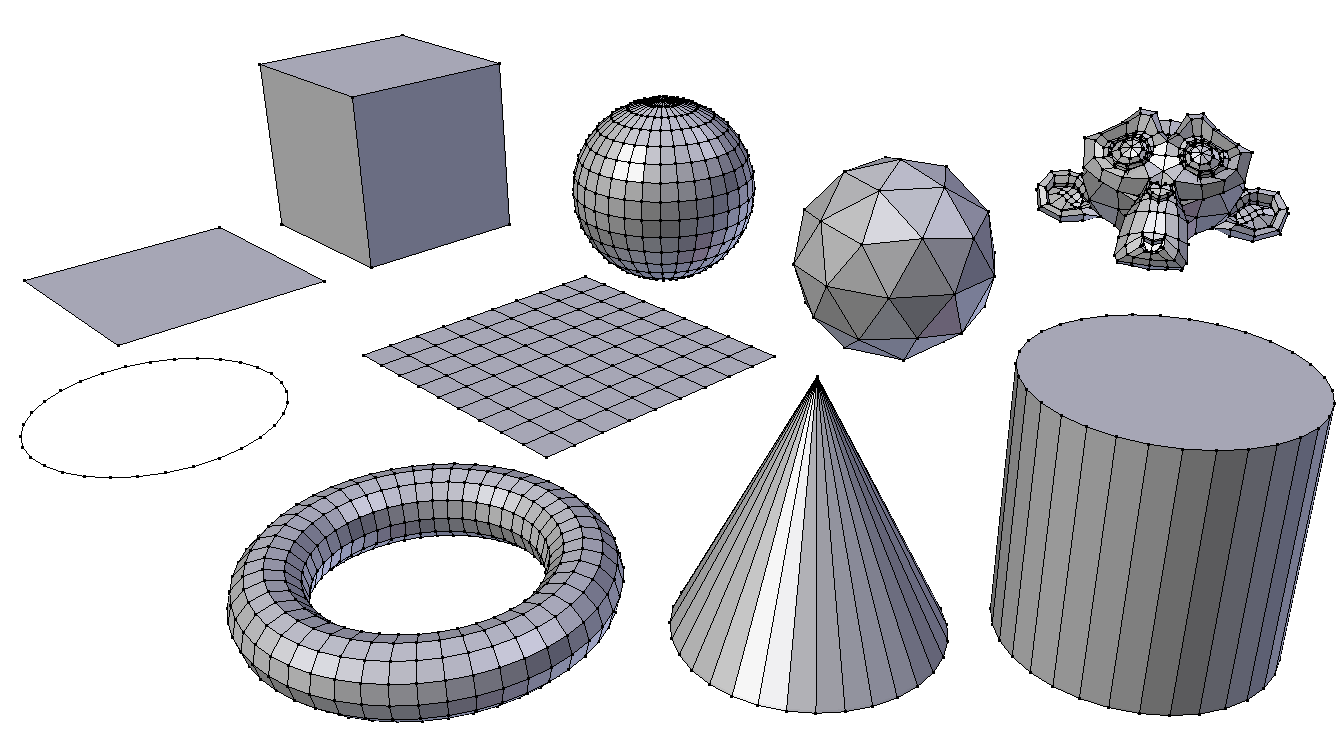
\includegraphics[width=14cm]{Img/GEO/geo-blender.png}
\centering
\caption{\textbf{ \footnotesize{Conjunto de primitivas 2D y 3D disponibles en Blender.}}}
\end{figure}


\subsubsection{Geometría non-manifold en Blender}

Se considera \textbf{non-manifold} una geometría que no puede ser representada en el mundo real, una malla non-manifold puede tener uno o más elementos con las siguientes propiedades:

\begin{enumerate}
    \item Una arista que une a más de dos caras.
    \item Dos o más caras conectadas solo por un vértice y no por una arista.
    \item Caras adyacentes cuyas normales apuntan en direcciones opuestas.
\end{enumerate}

\begin{figure}[h]
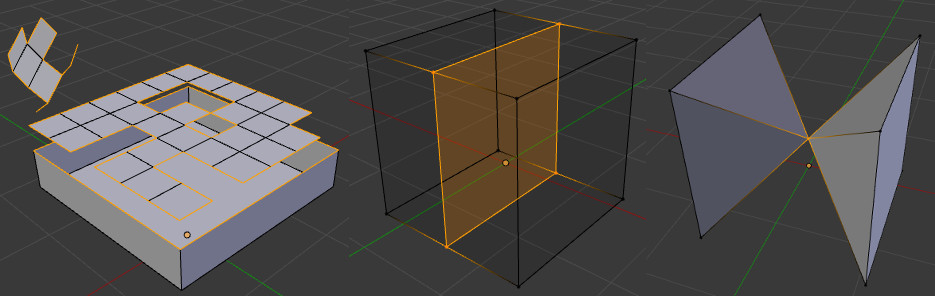
\includegraphics[width=12cm]{Img/Modelos/modelado20.jpg}
\centering
\caption{\textbf{ \footnotesize{Objetos no sólidos por geometria non-manifold en Blender. Caras y vértices sin conectar, Caras en el interior, Superficies sin grosor.}}}
\end{figure}


Para explicar una solución se utiliza la Figura \ref{fig:blender}. El modelo 3D de la izquierda no consiste en un volumen completo, sino en una serie de superficies que no están cerradas. Para garantizar que el objeto sea sólido es importante cerrar los agujeros en el modelo. Esto es posible creando una superficie con $N$ caras para tapar los agujeros como se puede apreciar en el resultado de la derecha.

\begin{figure}[h]
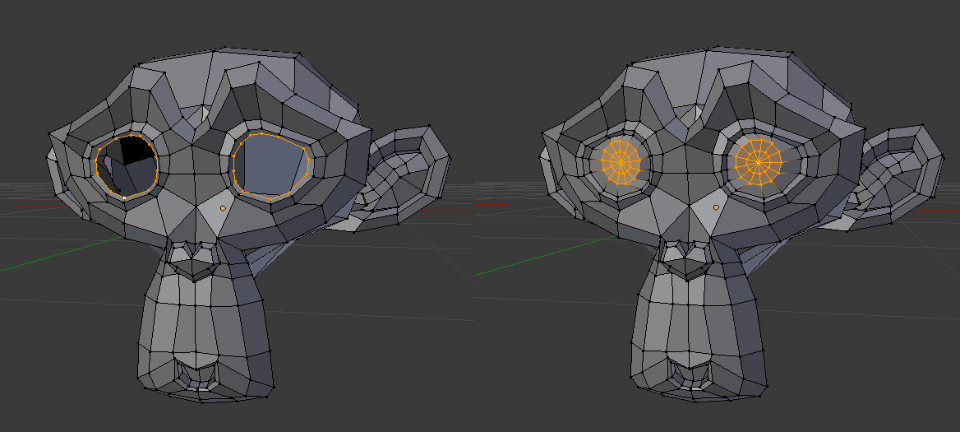
\includegraphics[width=10cm]{Img/Modelos/modelado21.jpg}
\centering
\caption{\textbf{ \footnotesize{Objeto no sólido por superficies no cerradas (izquierda)  y su solución incorporando caras  para cerrar los agujeros (derecha) }}}
\label{fig:blender}
\end{figure}

\subsubsection{Modelado booleano en Blender}

La recomendación en Blender para realizar operaciones booleanas es usar un \textbf{Modificador\footnote{
Los modificadores en Blender son operaciones automáticas que afectan a un objeto de una manera no destructiva.} Booleano} con el fin de tener mayor flexibilidad y realizar ediciones no destructivas\footnote{El método de edición no destructivo permite conservar la información geométrica que compone un modelo y así poder corregir errores y realizar cambios durante cualquier fase del proyecto}. Mediante los modificadores se pueden modificar los objetos y visualizar el operador booleano (union, intersección o diferencia) aplicado de forma interactiva y en tiempo real.

\begin{figure}[h]
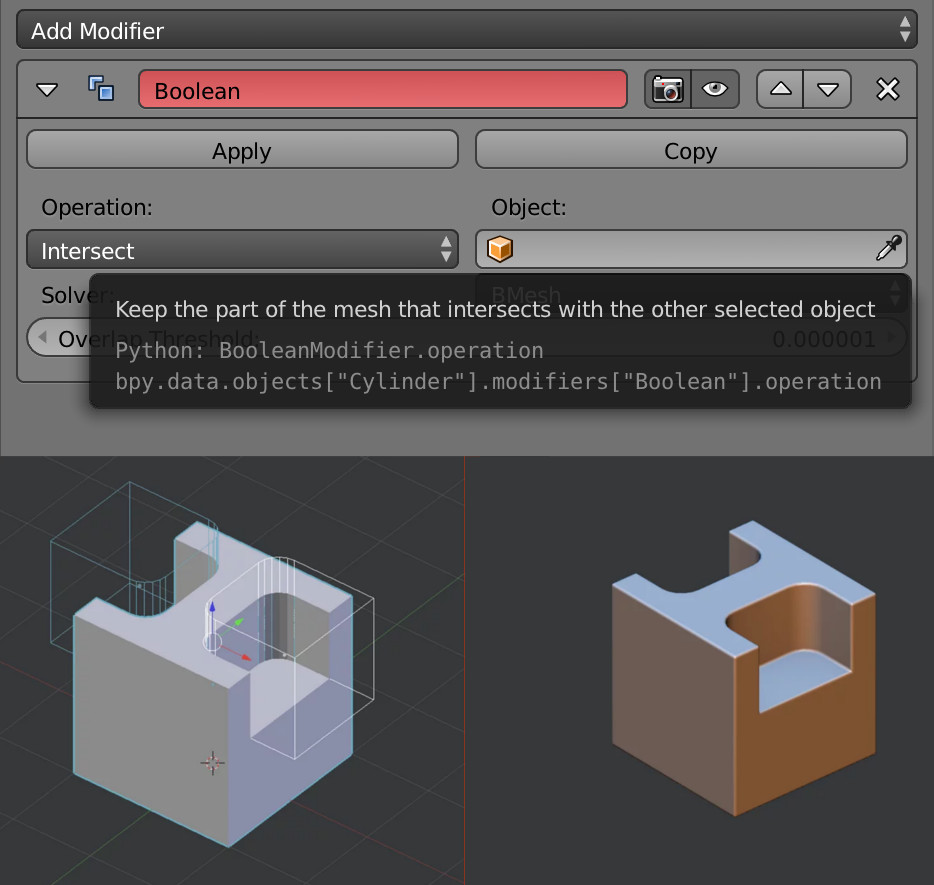
\includegraphics[width=9cm]{Img/Modelos/modelado22.jpg}
\centering
\caption{\textbf{ \footnotesize{Modificador booleano, aplicación de intersecciones y su resultado. }}}
\end{figure}

La herramienta booleana nativa de Blender es muy útil para partes simples (pocos polígonos) o para modelado mecánico. Con extensiones en inglés \textit{add-ons}\footnote{Un Add-on se entiende, del inglés, como una extensión o añadidura son programas que sólo funcionan anexados a otro y que sirven para incrementar o complementar sus funcionalidades} se puede extender la aplicación booleana a modelos con mallas complejas (con milones de polígonos) y que requieren una elevada potencia de cálculo.
\textbf{Cork}\footnote{\url{https://github.com/dfelinto/cork-on-blender}} es un complemento para Blender que se desarrolló especialmente para el ámbito de la impresión 3D. En la Figura \ref{fig:cork} se puede ver un ejemplo de su potencia en operaciones booleanas aplicado a casos reales de medicina.

\begin{figure}[h]
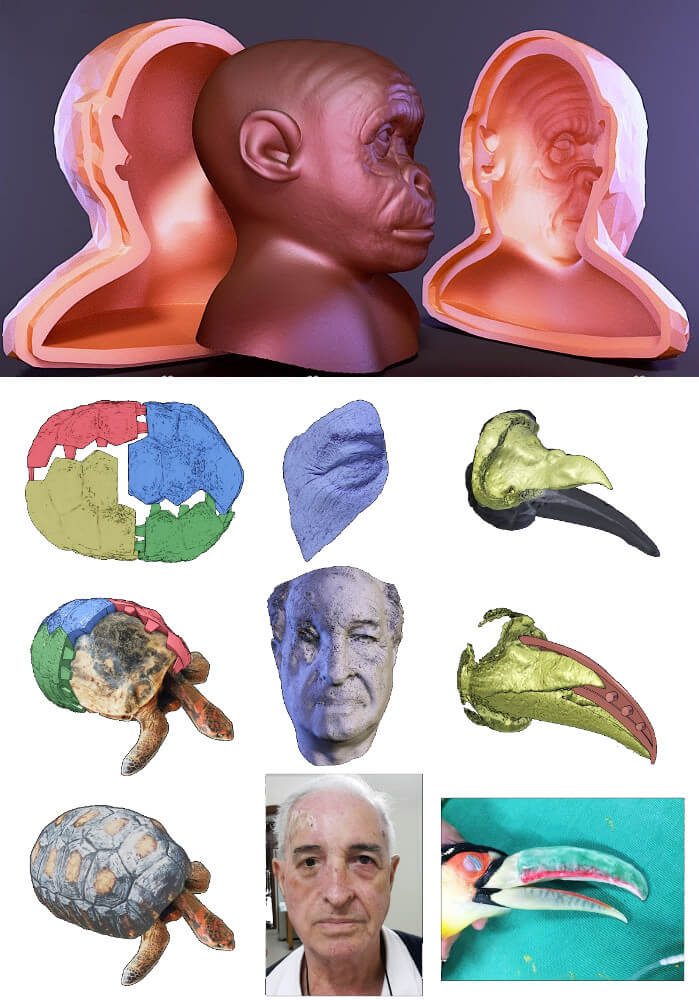
\includegraphics[width=12cm]{Img/Modelos/corkc.jpg}
\centering
\caption{\textbf{ \footnotesize{Ejemplo de modificadores booleanos con el add-on Cork y aplicaciones reales de prótesis médicas.   }}}
\label{fig:cork}
\end{figure}





\clearpage

\subsection{Programas para CAD especificado en algoritmos}
Las interfaces de scripting explicadas en la secciónXX, utilizadas para definir diseños paramétricos se puede encontrar en programas como \textbf{OpenSCAD}\footnote{\url{http://www.openscad.org/}}, una aplicación FLOSS para crear objetos sólidos de CAD utilizando geometría constructiva de sólidos (CSG).

\textquote{\textit{A diferencia de la mayoría del software libre para crear modelos 3D (como Blender), no se enfoca en los aspectos artísticos del modelado 3D sino en los aspectos CAD. Por lo tanto, podría ser la aplicación que está buscando cuando planea crear modelos 3D de partes de máquinas, pero que seguramente no está buscando cuando está más interesado en crear películas animadas por computadora.
OpenSCAD no es un modelador interactivo. En cambio, es algo así como un compilador 3D que lee un archivo de script que describe el objeto y representa el modelo 3D a partir de ese archivo. Esto le brinda a usted (el diseñador) un control total sobre el proceso de modelado y le permite cambiar fácilmente cualquier paso en el proceso o realizar diseños que están definidos por parámetros configurables}} \citep{Kintel}.
Un documento de OpenSCAD especifica primitivas geométricas y define como son modificadas y manipuladas para reproducir un modelo 3D.

En la última década se ha visto la aparición de un nuevo tipo de interfaz de secuencias de comandos, la interfaz visual. La programación visual implica representar programas no como texto, sino como diagramas. Un ejemplo es \textbf{Grasshopper}\footnote{ \url{http://www.grasshopper3d.com/}}, \textquote{\textit{editor de algoritmos gráficos estrechamente integrado con las herramientas de modelado 3-D de Rhino}} \citep{BobMcNeel}. Grasshopper se basa en gráficos que mapean el flujo de relaciones desde parámetros, a través de funciones definidas por el usuario, concluyendo normalmente con la generación de geometría. Los cambios en los parámetros o las relaciones del modelo hacen que los cambios se propaguen a través de las funciones explícitas para volver a dibujar automáticamente la geometría. Como tal, son otra forma de crear un modelo paramétrico.


\begin{figure}[h]
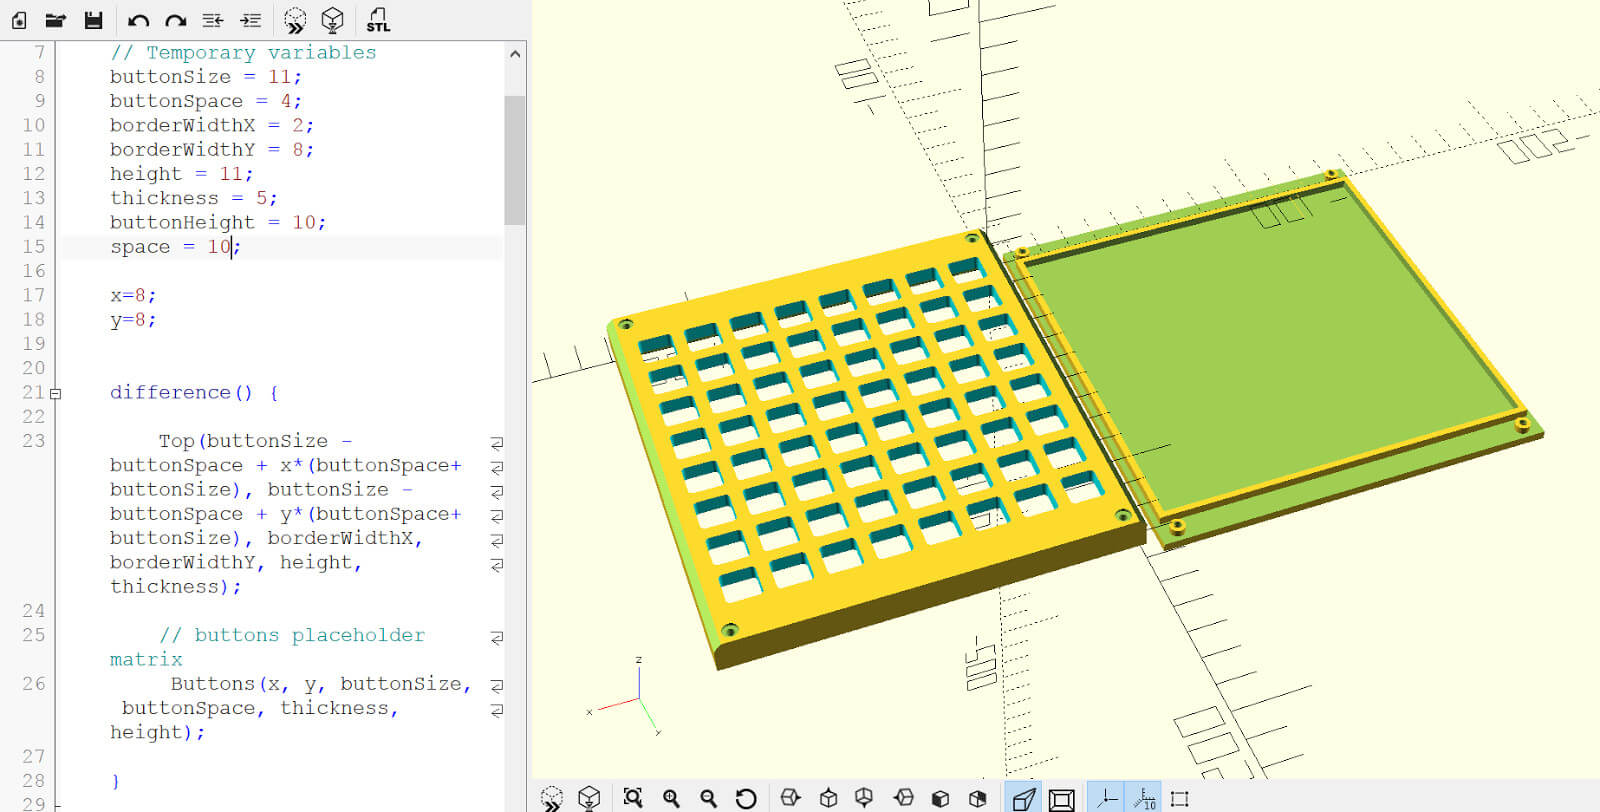
\includegraphics[width=14cm]{Img/CPD/openscadc.jpg}
\centering
\caption{\textbf{\footnotesize{Interfaz de OpenSCAD con el código que genera el modelo 3D}}}
\end{figure}

\begin{figure}[h]
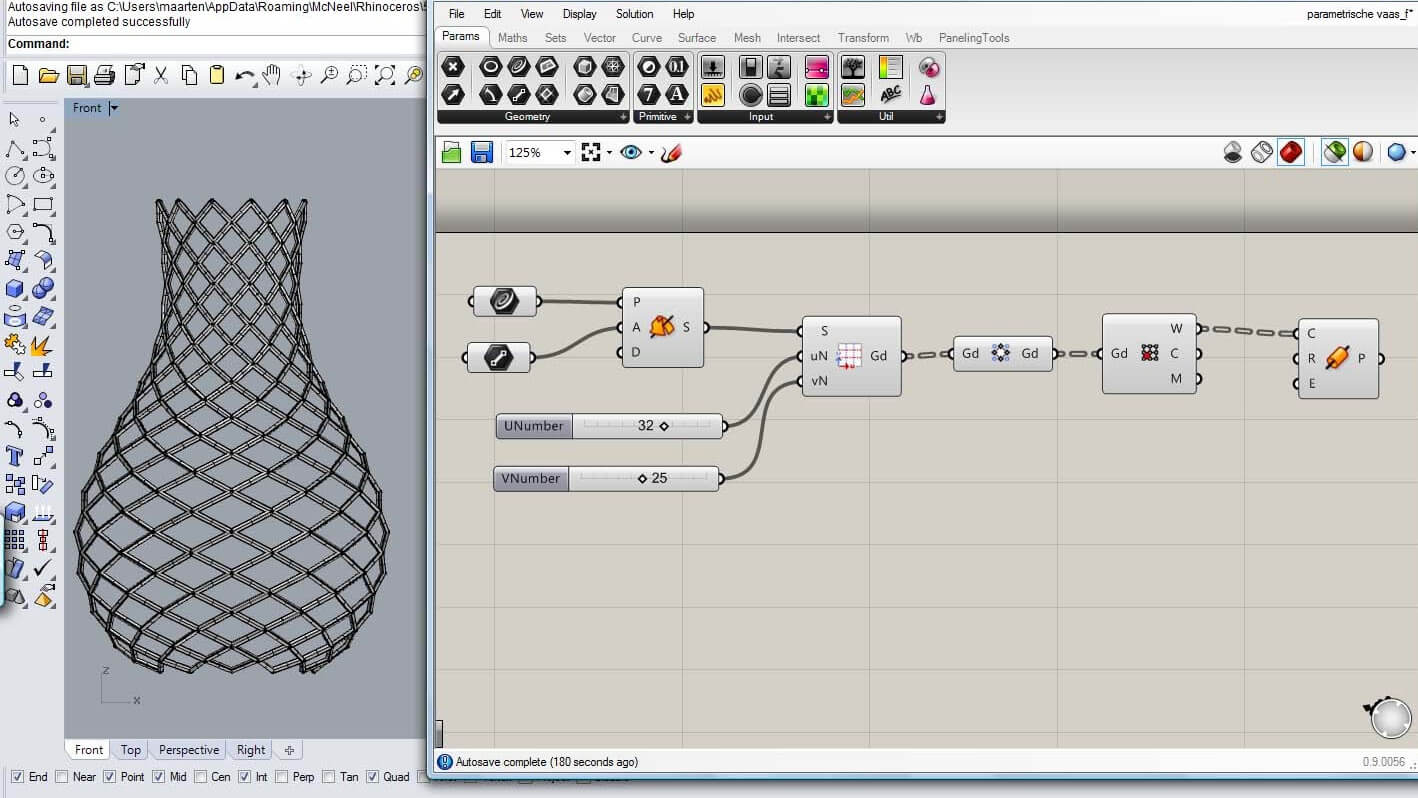
\includegraphics[width=14cm]{Img/CPD/rhinoc.jpg}
\centering
\caption{\textbf{\footnotesize{Rhinoceros con Graphopper, a la derecha se puede ver el diagrama que genera el modelo 3D}}}
\end{figure}




\subsection{Gráficos 3D en la web.}

\textquote{\textit{Las aplicaciones web se están volviendo cada vez más sofisticadas y la funcionalidad que alguna vez fue exclusiva de las aplicaciones de escritorio ahora también se puede encontrar en las aplicaciones web. Uno de los avances más recientes en este campo es la capacidad de las aplicaciones web para representar gráficos en 3D. Junto con el creciente número de dispositivos con procesadores gráficos y la capacidad de las aplicaciones web para ejecutarse en diferentes plataformas utilizando una única base de código, esto representa una posibilidad nueva y emocionante para los desarrolladores de aplicaciones gráficas en 3D}} \citep{Waerner2012}.

Además, el usuario final no tiene que instalar el software en su dispositivo para usarlo, esto se realiza automáticamente mediante el navegador web y cualquier complemento asociado. En general, las aplicaciones web ofrecen a los desarrolladores la oportunidad de llegar a una gran audiencia sin muchas dificultades a la hora de soportar múltiples plataformas, como sí sucedía anteriormente con las aplicaciones de escritorio. \vskip

Incluir gráficos 3D en aplicaciones web no es una nueva tendencia. En 1994, se estandarizó una forma de presentar escenas 3D en el navegador web a través de un lenguaje de marcado llamado \textbf{VRML}\footnote{\url{https://www.w3.org/MarkUp/VRML/}}. VRML permite que las escenas 3D se especifiquen en un lenguaje similar al HTML. Si bien hay (o ha habido) aplicaciones de nicho que usan VRML, hoy en día existen pocos sitios populares que incluyen documentos VRML. Parece haberse convertido en un estándar que nunca creció lo suficientemente ni se utilizo demasiado como para ver un uso significativo a gran escala. Es probable que el motivo fué la potencia de procesamiento disponible, sobre todo en computadoras de precios razonables, que en esa época no fueron lo suficientemente potentes para proporcionar gráficos 3D convincentes. Esto ha cambiado recientemente con procesadores gráficos dedicados que se abren paso en más y más tipos de dispositivos. Gracias a esto, ha habido un renovado interés en las tecnologías que proporcionan gráficos 3D en páginas web y en aplicaciones web.\vskip

Los gráficos 3D interactivos son una de las áreas más grandes e importantes donde las aplicaciones web no tuvieron mucho éxito hasta hace poco. Parte de esto se debe a que este tipo de interactividad exige comprometer en gran parte del dispositivo y el software relacionado, como las máquinas virtuales para lenguajes de scripting tan a menudo involucradas en este tipo de aplicaciones. Otra razón fué la falta de una Interfaz de Programación de Aplicaciones en inglés  \textit{Application Programming Interface} (API) para gráficos 3D en la mayoría de las tecnologías de aplicaciones web. Ambas áreas han visto mejoras, la primera con técnicas tales como compilación \textbf{just-in-time} (JIT)\footnote{Un compilador JIT (Just-In-Time) es un componente de software que mejora el rendimiento de las aplicaciones compilando códigos de bytes en código de máquina nativa, en tiempo de ejecución. } y la segunda con la introducción de tecnologías como Stage 3D para Flash\footnote{\url{https://www.adobe.com/devnet/flashplayer/stage3d.html}} y WebGL. 
\vskip

La realidad de las aplicaciones actuales implica que las soluciones sean capaces de ejecutarse en más plataformas, admitir más navegadores y dispositivos, por lo tanto, se vuelve fundamental elegir una tecnología desde una perspectiva de compatibilidad, como WebGL. La Figura \ref{fig:compa} muestra la compatibilidad de WebGL con los navegadores más utilizados y sus respectivas versiones.

\begin{figure}[h]
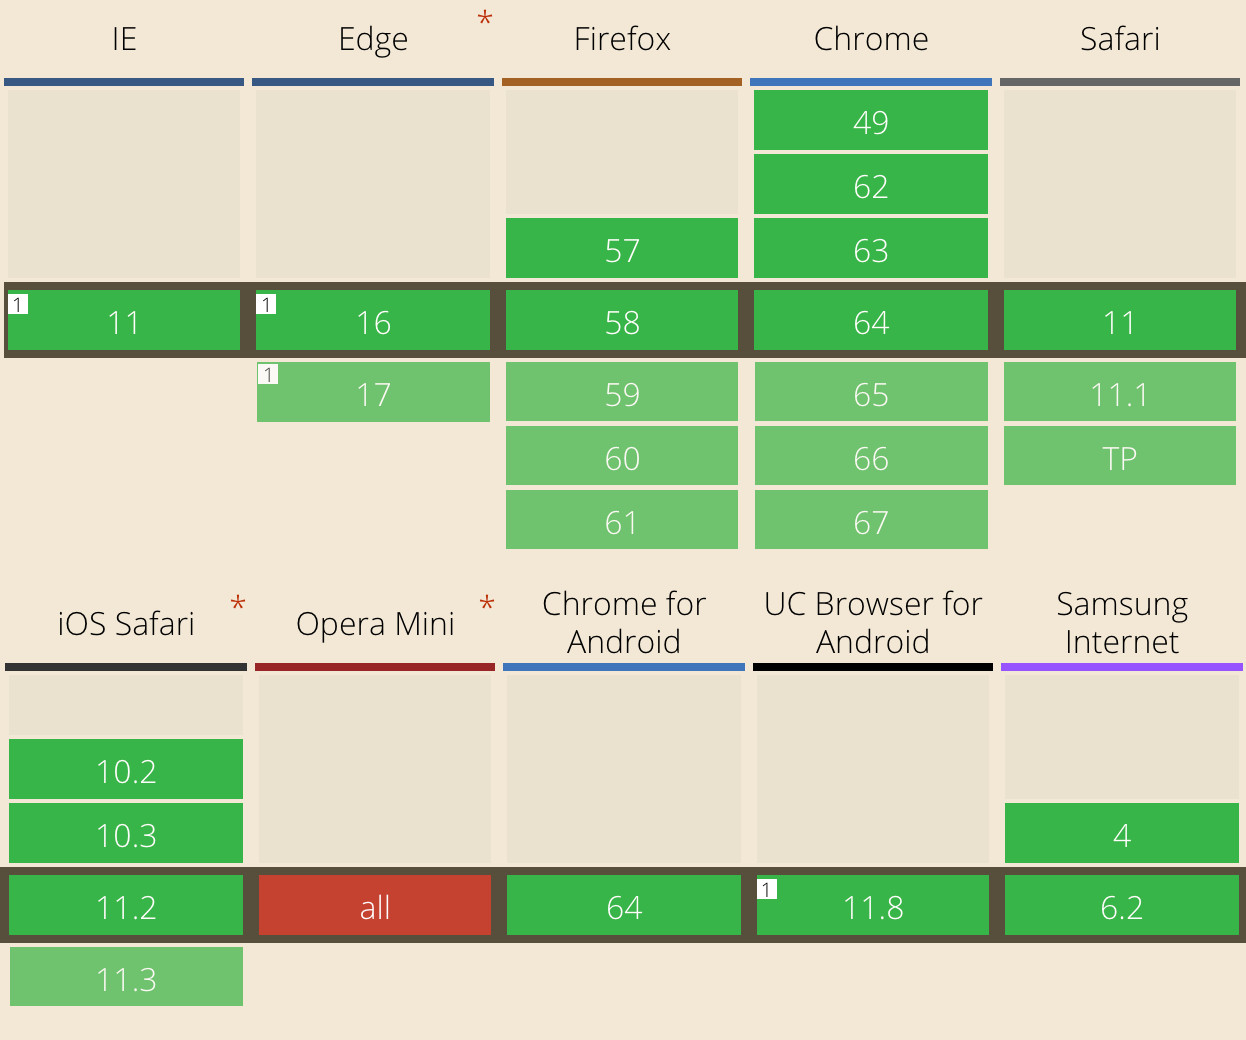
\includegraphics[width=16cm]{Img/WEB/web-compa.jpg}
\centering
\caption{\textbf{\footnotesize{Compatibilidad de WebGL con navegadores web. Verde (Soportado) y Rojo (No soportado). Fuente \url{https://caniuse.com/} }}}
\label{fig:compa}
\end{figure}


\subsubsection{WebGL}
\textquote{\textit{\textbf{WebGL}\footnote{\url{https://www.khronos.org/webgl/}} es una API multiplataforma y libre de regalías utilizada para crear gráficos 3D en un navegador web}} \citep{KronosGroup}. 
WebGL en inglés \textit{Web Graphic Library}  es una API de JavaScript de ``bajo nivel'' desarrollada por la fundación Mozilla en 2006, con la intención de proporcionar una API de gráficos 3D para el elemento canvas\footnote{\url{https://developer.mozilla.org/es/docs/Web/HTML/Canvas}} de HTML. La especificación WebGL es mantenida desde el 2009 por Khronos Group. A pesar de no ser parte de la especificación oficial de HTML5, en la actualidad es compatible con todos los principales navegadores y se ha convertido en la API estándar para gráficos 3D en navegadores. \vskip 

\textquote{\textit{``Bajo nivel'' significa que los comandos WebGL se expresan en términos que se relacionan de manera relativamente directa a cómo funciona realmente una GPU (unidad de procesamiento de gráficos, es decir, hardware). Eso significa que WebGL permite aprovechar realmente el conjunto de características y la potencia de las tarjetas gráficas. Lo que los juegos nativos hacen mediante OpenGL o Direct3D, probablemente también lo hagan con WebGL.
WebGL es de tan bajo nivel que ni siquiera es una API de gráficos ``3D'', hablando correctamente. Al igual que a al hardware gráfico no le importa si está haciendo gráficos 2D o 3D, tampoco WebGL: \textbf{2D y 3D son solo dos posibles patrones de uso}}} \citep{Nyman2013}.

\vskip Cuando OpenGL 1.0 salió en 1992, era específicamente una API 3D, con el objetivo de exponer las características del hardware de gráficos 3D de esa época, a medida que éste fué evolucionando para ser más genérico y programable, también lo hizo OpenGL. Eventualmente, OpenGL se volvió tan genérico que el 2D y 3D son solo dos casos de uso posibles, a la vez que ofrecen un gran rendimiento. Ese fué el caso de OpenGL 2.0, y WebGL siguió ese concepto en su desarrollo.

A eso se refiere la definición de WebGL como una API de gráficos de bajo nivel en lugar de una API 3D específica. 

Sin embargo, la naturaleza genérica de WebGL hace que desarrollar en contextos de gráfica sea una tarea engorrosa, como se puede apreciar en la documentación oficial de la API y tutoriales de la comunidad \citep{MozillaFoundation}. Para solventar este hecho, se construyeron frameworks y librerías con WebGL como base para proporcionar una interfaz de más alto nivel para la API. Las opciones de software para desarrollar gráficas en la web son muy variadas, desde representación de gráficos vectoriales escalables en inglés \textit{Scalable Vector Graphics} (SVG)\footnote{\url{https://www.w3.org/Graphics/SVG/}} hasta realidad virtual con WebVR\footnote{\url{https://webvr.info/}}. A continuación se analizan y evalúan dos de estas tecnologías, que se consideran técnicamente aptas para cumplir con los objetivos de desarrollo de este trabajo: \textbf{OpenJSCAD} y \textbf{Three.js}.

\subsubsection{OpenJSCAD}
OpenJSCAD\footnote{\url{https://openjscad.org/}}
\textquote{\textit{es un conjunto de herramientas modulares para diseños paramétricos 2D y 3D, que pueden ejecutarse en el navegador web y a través de interfaces de linea de comandos mediante código JavaScript}} \citep{ReneK.MuellerJeffGay}. 
OpenJSCAD es un proyecto que tiene como objetivo implementar funcionalidades de OpenSCAD utilizando tecnologías web. En lugar de utilizar el lenguaje de OpenSCAD, se utiliza JavaScript. 
A continuación algunas características:

\begin{itemize}
    \item Se puede ejecutar en el navegador web sin necesidad instalar ningún software extra.
    \item Se puede instalar todas las capacidades de la web oficial del proyecto en un servidor propio.
    \item Posee una Interfaz de linea de comandos en inglés \textit{Command Line Interface} (CLI) para computar los modelos en el servidor con Node.js.
    \item Se visualiza en el navegador mediante webGL, haciendo uso de canvas de HTML5.
    \item Soporta modelos paramétricos con parámetros editables por el usuario sin la necesidad de editar el script de origen.
    \item Soporta modelado booleano CSG y transformaciones geométricas.
    \item Los sólidos se almacenan en variables. Esto permite, permite operaciones como la clonación de objetos.
    \item Amplio soporte para matemáticas 2D y 3D (clases para Vector2D, Vector3D, Plane, Line3D, Line2D).
    \item Los sólidos 3D se puede exportar a archivos STL, las áreas 2D se pueden exportar con archivos DXF. También permite la importación en ambos casos.
\end{itemize}

Para trabajar con modelado booleano OpenJSCAD utiliza una librería llamada \textbf{CSG.js} \footnote{\url{https://github.com/jscad/csg.js}}, \textquote{\textit{esta librería implementa operaciones CSG en las mallas de forma elegante y concisa usando \textbf{BSP trees} y su objetivo es funcionar como una implementación fácilmente comprensible de ese algoritmo}} \citep{Nieuwenhuijse}.
La Partición Binaria del Espacio en ingles \textit{Binary Space Partitioning} (BSP) es un método para subdividir recursivamente un espacio en elementos convexos empleando hiperplanos. Esta subdivisión da lugar a una representación de la escena por medio de una estructura de datos de árbol conocida como árbol de BSP en inglés \textit{BSP trees}. 

OpenJSCAD hace que su funcionalidad esté disponible como funciones y métodos a través de sus objetos, y por ende que los programas escritos sean más flexibles. Esto permite al programador utilizar el paradigma de programación funcional\footnote{La programación funcional es un paradigma de programación declarativa basado en el uso de funciones, en contraste con la programación imperativa, que enfatiza los cambios de estado mediante la mutación de variables} y facilita la comprensión de los programas escritos. El paradigma que utiliza la librería se explica con mas detalle en la sección XXX de desarrollo de este trabajo.

OpenJSCAD para la visualización utiliza como base \textbf{}lightgl.js \footnote{\url{https://github.com/evanw/lightgl.js/}}, \textquote{\textit{esta librería facilita el prototipado rápido de aplicaciones WebGL. Lo hace en un nivel más bajo que muchas otras bibliotecas WebGL y aunque no proporciona un \textbf{scene graph}, re-implementa la matriz modelo-vista/proyección\footnote{\url{http://www.opengl-tutorial.org/es/beginners-tutorials/tutorial-3-matrices/}} de OpenGL para proporcionar una funcionalidad similar}} \citep{Wallace}.\vskip
Un gráfico de escena en inglés \textit{Scene Graph}\footnote{\url{https://en.wikipedia.org/wiki/Scene_graph}} es una estructura de datos general comúnmente utilizada por aplicaciones de edición de gráficos basadas en vectores y juegos de computadora modernos, que organiza la representación lógica y a menudo espacial de una escena gráfica.

\vspace{5mm}
\textbf{Creación de un cubo con OpenJSCAD}

Un script OpenJSCAD debe tener al menos una función definida, la funcion \textit{main()}, que retorna un objeto CSG o un vector (array) de dos o más objetos CSG. En el siguiente ejemplo se crea un cubo de color azul con código OpenJSCAD, se puede ver el resultado en la Figura \ref{fig:jopen}. 

\begin{minted}[baselinestretch=1, bgcolor=LightGray, linenos]{js}
 function main() {
     // Cubo de tamaño 20 de color azul
     return cube({size: 20}).setColor([0, 0, 1]);
 }
\end{minted}

\begin{figure}[h]
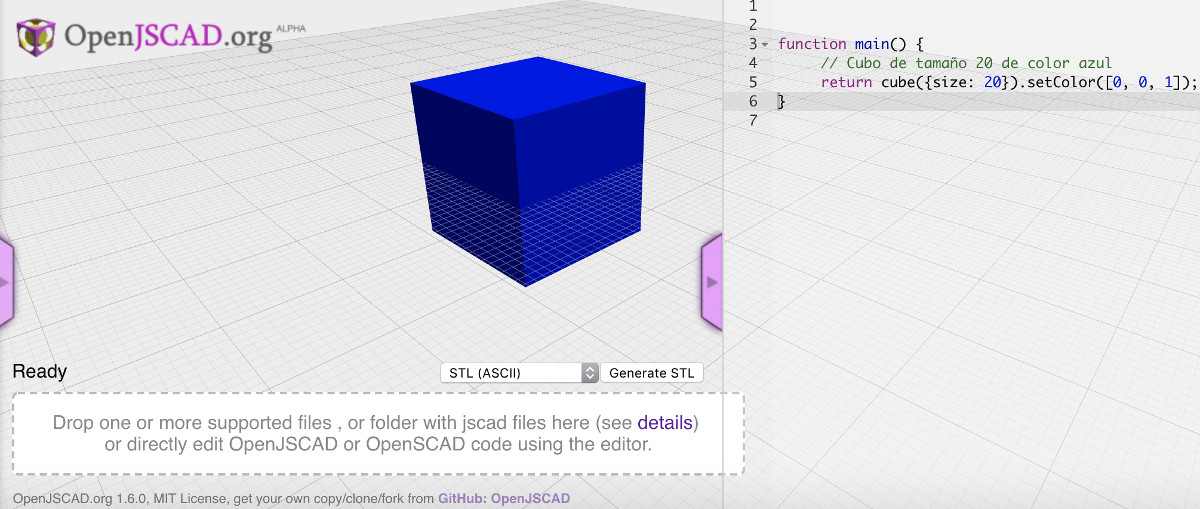
\includegraphics[width=15cm]{Img/WEB/web-jopen.jpg}
\centering
\caption{\textbf{\footnotesize{Interfaz de OpenJSCAD }}}
\label{fig:jopen}
\end{figure}


\clearpage
\subsubsection{Three.js}
Three.js\footnote{\url{https://threejs.org/}} es una librería/API desarrollada en JavaScript y soportada en la mayoría de los navegadores web. Es utilizada sobre todo para crear y visualizar gráficos 3D animados en los navegadores web. Los scripts de Three.js se pueden utilizar mediante canvas de HTML5, SVG o WebGL. Contiene abstracciones de alto nivel para tareas comunes de WebGL y proporciona, entre otras capacidades, las siguientes:

\begin{itemize}
    \item Se puede ejecutar en el navegador web sin necesidad instalar ningún software extra.
    \item Se puede instalar utilizando NPM y Node.js.
    \item Capacidad de gestionar objetos en un escena.
    \item Render usando WebGL, SVG o incluso CSS (con el propósito de soportar navegadores sin soporte de WebGL).
    \item Matemáticas relacionadas con 3D, marcadores de fronteras, transformaciones en objetos de la escena.
    \item Trabajar con una gran cantidad de objetos predefinidos como Primitivas, Materiales (shaders), Luces, Cámaras.
    \item Efectos gráficos como desenfoque de cámara.
    \item Cargadores para archivos de modelos 3D como Collada, STL, Obj.
    \item Puede trabajar con audio mediante WebAudio API\footnote{\url{https://developer.mozilla.org/es/docs/Web_Audio_API}}.
    \item Animación por keyframes usando esqueletos y otros sistemas.
    \item Simulaciones físicas como colisiones, telas, iluminación realista.
\end{itemize} 

\subsubsection{Creación de un cubo con Three.js}

Para poder mostrar algo realmente  con three.js, se necesitan tres cosas: \textit{escena, cámara y renderizador}. Esto es obligatorio para poder renderizar la escena mediante la cámara. En el siguiente ejemplo se crea un cubo azul con código Three.js. 

\begin{minted}[baselinestretch=1, bgcolor=LightGray, linenos]{js} 

 // Se crea una escena
 scene = new THREE.Scene();

 // Se crea una cámara
 camera = new THREE.PerspectiveCamera();
 camera.position.x = 0;
 camera.position.y = 0;
 camera.position.z = 60;
	
 // Se agrega la cámara a la escena		
 scene.add( camera );

 // Se crea un material de color azul			
 var material= new THREE.MeshBasicMaterial( { color: 0x0000ff } );
 // Se crea un cubo de tamaño 20, con el material de color azul 
 cube = new THREE.Mesh( new THREE.CubeGeometry( 20, 20, 20 ), 
 material );
 // Se agrega el cubo a la escena
 scene.add( cube );


 // Se crea un renderizador
 renderer = new THREE.CanvasRenderer();

 // Se realiza el render de la escena con la cámara
 renderer.render( scene, camera );

\end{minted}

Three.js utiliza el concepto de gráfico de escena en inglés \textit{Scene Graph}. La mayoría de los motores 3D usan este concepto, se colocan los objetos que se necesitan visualizar en el gráfico de escena. El motor recorre el gráfico de la escena y calcula una lista de elementos para dibujar. Un gráfico de escena es una colección de nodos en estructura de árbol jerárquico.

Una escena es un soporte para todos los objetos que componen un mundo en 3D, incluidas las luces, los objetos gráficos y posiblemente las cámaras. Actúa como un nodo raíz para el gráfico de escena. Una cámara es un tipo especial de objeto que representa un punto de vista desde el cual se puede hacer una imagen de un mundo 3D. Representa una combinación de una transformación de visualización y una proyección. Un procesador es un objeto que crea la imagen. Los renderizadores siempre dibujarán la imagen en un canvas de HTML.

\begin{figure}[h]
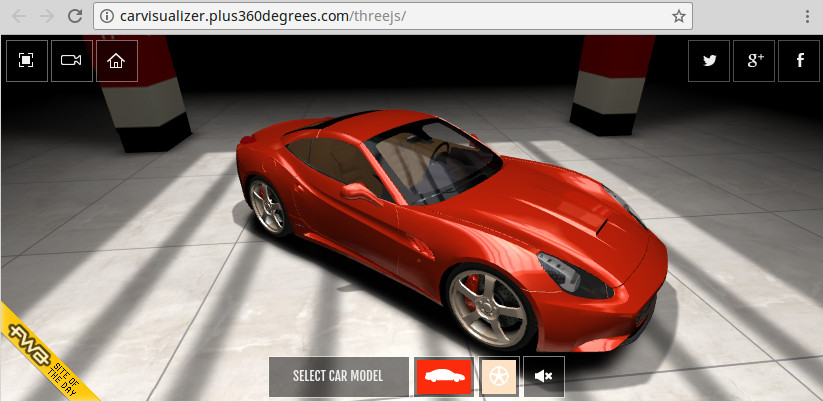
\includegraphics[width=15cm]{Img/WEB/web-three.jpg}
\centering
\caption{\textbf{\footnotesize{Ejemplo de aplicación con Three.js fuente: \url{http://carvisualizer.plus360degrees.com/threejs/} }}}
\label{fig:threejs}
\end{figure}

\clearpage
\subsubsection{Evaluación} \textcolor{red}{Ver si poner en desarrollo}

A continuación en la tabla se analizan las librerías OpenJSCAD y Three.js respecto a los requerimientos del prototipo CoCADA.

\begin{center}
 \begin{tabular}{ c |c c } 
   \empty & OpenJSCAD & Three.js  \\ 
   \hline
   Enfoque de modelado booleano CSG & Sí & No \\
   \hline
   Visualizacion vía WebGL & Sí & Sí \\
   \hline
   Implementación de Ray Tracing & Sí & Sí \\
   \hline
   Interfaz CLI & Sí & No \\
   \hline
   Compatibilidad con la mayoría de los navegadores & Sí & Sí \\
   \hline
   Importación/Exportación de otros formatos & Sí & Sí \\
   \hline
   
   
\end{tabular}
\end{center}
\vskip
\begin{center}
\caption{Tabla comparativa entre OpenJSCAD y Three.js}
\end{center}

Si bien las funcionalidades de ambas tecnologías pueden ser similares, es importante aclarar el ámbito de aplicación de cada una respecto al prototipo.

\begin{itemize}
    \item OpenJSCAD es un conjunto de herramientas que permiten resolver el modelado mediante scripting en la web, con una calidad de visualización suficiente para poder comprender la geometría de un modelo sólido.
    \item Three.js es una librería que puede realizar modelado booleano mediante plugins\footnote{Los plugins son herramientas que extienden la funcionalidad de un software}, sin embargo se utiliza normalmente para crear complejas visualizaciones y animaciones en 3D. Es una herramienta conocida videojuegos, aplicaciones interactivas, obras de arte digital, instalaciones para productos, etc. Explotando las posibilidades como la iluminación, las simulaciones físicas, el uso de cámaras, las partículas, la interacción con dispositivos y el trabajo con audio.
\end{itemize}

 En definitivas, los ámbitos de aplicación de estas dos tecnologías son diferentes. Con OpenJSCAD se obtienen herramientas de forma casi directa para resolver los requerimientos del prototipo, mientras que con Three.js se debe adaptar su lógica de funcionamiento a un ámbito mucho más acotado en términos de funcionalidad y visualización. Por todo lo mencionado se considera que OpenJSCAD es la opción indicada para ser utilizada en el desarrollo del prototipo COCADA.
 

\textcolor{red}{Inspirado en Using 3D functionality available in current web-browsers to create and visualize geological}

EJ..
\begin{itemize}
    \item 2.1 WebGL
    \item 2.2 Choosing a graphics framework/library 2.2.1 Three.js
    \item 2.2.2 X3DOM and X3D
    \item 2.3 Web application frameworks \item 2.3.1 Angular \item 2.3.2 Reac
\end{itemize}



\clearpage
\subsection{Intercambio de datos en la web}

En la actualidad los sistemas PDM están aprovechando las posibilidades que ofrece internet. Este nuevo enfoque permite el trabajo entre personas establecidas en distintos puntos geográficos, gracias a la posibilidad de acceso remoto a las bases de datos. 
Con estos nuevos sistemas es posible la utilización del PDM por parte de múltiples especialistas implicados en el desarrollo de un producto, permitiendo que esta tecnología sea una plataforma de integración entre los interesados y una excelente ayuda para el workflow\footnote{El flujo de trabajo en inglés \textit{workflow} es el estudio de los aspectos operacionales de una actividad de trabajo} en el diseño de productos.


A continuación se explican brevemente los dos formatos más utilizados para Data Exchange en contextos web, el tradicionalmente utilizado (XML) y (JSON) comparativamente nuevo, sus objetivos de diseño y sus características fundamentales.

\subsubsection{XML}

\textquote{\textit{XML\footnote{\url{https://www.w3.org/XML/}} o Extensible Markup Language es un conjunto de estándares publicados por XML Working Group en el Consorcio World Wide Web  (W3C), el grupo que regula los estándares de Internet (www)}} \citep{Zunke2014}. Básicamente, un documento XML se compone de algunas etiquetas, en inglés \textit{tags} bien definidas y los datos incluidos en ellas. Las etiquetas son contenedores que describen los datos adjuntos y también los organizan. Los objetivos de diseño para XML v1.1 publicados en la recomendación W3C son los siguientes:

\begin{itemize}
    \item XML se podrá usar directamente en Internet.
    \item XML debe admitir una amplia variedad de aplicaciones.
    \item XML debe ser compatible con SGML.
    \item Será fácil escribir programas para procesar documentos XML.
    \item El número de características opcionales en XML debe mantenerse en el mínimo absoluto, idealmente cero.
    \item Los documentos XML deben ser legibles por los humanos y razonablemente claros.
    \item El diseño de XML debe prepararse rápidamente.
    \item El diseño de XML debe ser formal y conciso.
    \item Los documentos XML deben ser fáciles de crear.
    \item La rigidez en el marcado XML es de mínima importancia.
\end{itemize}

La especificación de la sintáxis y las regulaciones con respecto a la correcta forma de un documento XML se pueden consultar en la especificación W3C para XML v1.1\footnote{\url{https://www.w3.org/TR/2006/REC-xml11-20060816/}}

\begin{minted}[baselinestretch=1, bgcolor=LightGray]{HTML}
<?xml version="1.1"?> 
    <greeting>Hola Mundo!</greeting> 
<!--Esto es un comentario -->
\end{minted}
\begin{center}
    \caption{Ejemplo de un documento XML}    
\end{center}



\subsubsection{JSON}
\textquote{\textit{JSON o Javascript Object Notation es un formato de datos abierto basado en texto ligero y diseñado para que los datos sean legibles por humanos}} \citep{Zunke2014}, el formato ha sido especificado y popularizado por el programador Douglas Crockford\footnote{\url{https://crockford.com/}}.

JSON está constituído por dos estructuras:

\begin{itemize}
    \item Una colección de pares de nombre/valor. En varios lenguajes esto es conocido como un objeto, registro, estructura, diccionario, tabla hash, lista de claves o un arreglo asociativo.
    \item Una lista ordenada de valores. En la mayoría de los lenguajes, esto se implementa como arreglos, vectores, listas o sequencias.
\end{itemize}

Estas son estructuras universales; virtualmente todos los lenguajes de programación las soportan de una forma u otra. Por ende, es razonable que un formato de intercambio de datos que es independiente de los lenguajes de programación se base en estas estructuras.

\begin{minted}[baselinestretch=1, bgcolor=LightGray]{HTML}
{ "greeting": "Hola Mundo!" } 
\end{minted}
\begin{center}
\caption{Ejemplo de objeto JSON}
\end{center}

\subsubsection{Comparación de características}
En esta sección se analizan y comparan las características más destacadas de ambos formatos.

\begin{enumerate}
    \item \textbf{Adopción en la Industria}
    \begin{itemize}
        \item XML ha sido el estándar de la industria por mas de una década y tiene muchos apoyo gracias a los estándares.
        \item JSON, por otro lado, si bien es ampliamente utilizado, no tiene estándares como Schematrons, XSD.
    \end{itemize}
    
    \item \textbf{Metadatos}
    \begin{itemize}
        \item XML tiene una gran sobrecarga en forma de metadatos por el uso de etiquetas \textless \textgreater.
        \item JSON tiene metadatos mínimos que lo hacen muy compacto.
    \end{itemize}
    
    \item \textbf{Soporte de frameworks}
    \begin{itemize}
        \item XML es compatible con la mayoría de las implementaciones de framework (API) en toda la industria.
        \item Al principio JSON no tenía mucho soporte, sin embargo pero se ha posicionado muy rápido en términos de adopción.
    \end{itemize}
    
    \item \textbf{Extensibilidad}
    \begin{itemize}
        \item XML permite almacenar cualquier tipo de datos. Los atributos del elemento de datos permiten flexibilidad adicional.
        \item JSON está limitado solo al almacenamiento de datos clásicos como texto y números.
    \end{itemize}
    
    \item \textbf{Facilidad de mapeo}
    \begin{itemize}
        \item XML está orientado a documentos (estructura de árbol), lo que dificulta su asignación a objetos en el paradigma de programación orientado a objetos (OOP).
        \item JSON está orientado a datos, por lo tanto, está más cerca de la estructura de los objetos en el paradigma de OOP.
    \end{itemize}
    
    \item \textbf{Rendimiento}
    \begin{itemize}
        \item Debido a la sobrecarga de metadatos, los datos requiere, de más ancho de banda si se expresan en XML.
        \item Los datos en JSON son muy compactos, utilizando la menor cantidad de ancho de banda.
    \end{itemize}
    
\end{enumerate}


\subsubsection{Análisis de rendimiento (Benchmark)}
Para el análisis y la comparación del rendimiento, ambos formatos de datos (XML y JSON) se comparan respecto al uso de memoria y los tiempos de ejecución en los siguientes 3 experimentos:
\begin{enumerate}
    \item Serialización o marshaling desde un objeto Java a una secuencia de memoria almacenada (buffer) sin compresión.
    \item Serialización o marshaling desde un objeto Java a una secuencia de memoria almacenada (buffer) con compresión.
    \item Des-serialización o unmarshaling de una secuencia de memoria almacenada (buffer) a un objeto Java.
\end{enumerate}

Las pruebas de rendimiento se realizaron ejecutando 100 muestras para cada experimento y 100 instancias de cada experimento. A continuacion se pueden ver muestras generadas de archivos XML y JSON respectivamente.

\begin{minted}[baselinestretch=1, bgcolor=LightGray]{HTML}
<?xml version="1.0" encoding="UTF-8" ?> 
<Hotel xmlns="http://www.example.org/Hotel">
    <hotelID>15013</hotelID>
    <hotelName>rhhjwhuqabhpitcewkrc</hotelName> 
    <menu> 
        <food> 
            <name>wdppncqtkhubtvkagpvm</name> 
            <price>48161</price> 
            <calories>49311</calories>
        </food>
    </menu>
</Hotel>
\end{minted}
\begin{center}
\caption{Archivo XML de muestra generado aleatoriamente}
\end{center}

\begin{minted}[baselinestretch=1, bgcolor=LightGray]{HTML}
{"hotelID":80814, "hotelName":"glovcnbwaviboawddgvx", 
"menu":
{"food":[{"name":"fprgunyzwvjkruwalbny",
"price":63463,"calories":95471}]}}
\end{minted}
\begin{center}
\caption{Archivo JSON de muestra generado aleatoriamente}
\end{center}


La siguiente tabla resume las medidas concluyentes de los experimentos. La medida del tiempo se establece en nanosegundos (ns) y la medida de memoria se establece en Bytes (B).

\begin{center}
 \begin{tabular}{ | c | c | c | c |} 
   \hline
   Aspectos de rendimiento & JSON & XML & JSON/XML  \\ 
   \hline
   Tamaño de Secuencia (sin comprimir) & 137B & 279B & 49\% \\
   \hline
   Tamaño de Secuencia (comprimido) & 133B & 219B & 61\% \\
   \hline
   Consumo en la Serialización & 3312B & 22128B & 15\% \\
   \hline
   Consumo en la Des-serialización & 5840B & 7040B & 83\% \\
   \hline
   Tiempo de Serialización (sin comprimir) & 11614ns & 23591ns & 49\% \\
   \hline
   Tiempo de Serialización (comprimido) & 9884ns & 19310ns & 51\% \\
   \hline
   Tiempo de Des-serialización & 13880ns & 43595ns & 32\% \\
   \hline
 
\end{tabular}
\end{center}
\begin{center}
\caption{\textbf{\footnotesize{Medidas concluyentes de los experimentos}}}
\end{center}

\textbf{Conclusiones}\vskip
En lo que respecta al rendimiento, el formato de intercambio de datos JSON es el claro ganador entre los dos. Tanto en términos de uso de memoria como de tiempo de ejecución, JSON ofrece un mejor rendimiento. Incluso con la compresión habilitada, XML produjo mucho más sobrecarga en la secuencia de datos que JSON.

\vspace{5mm}
XML se puede utilizar como data exchange si:
\begin{itemize}
    \item El rendimiento de la aplicación no es la principal prioridad.
    \item Se puede permitir que el consumo de memoria de una aplicación sea grande.
    \item Es necesario que haya un estricto cumplimiento de un protocolo estándar para la comunicación.
    \item La optimización de los datos enviados a través de la red no es prioridad.
\end{itemize}

Por el contrario, JSON se puede utilizar como data exchange si:
\begin{itemize}
    \item El rendimiento de la aplicación es una consideración de diseño.
    \item El tiempo de utilización de memoria de una aplicación debe mantenerse muy pequeño o mínimo.
    \item Puede haber una desviación sobre el formato de comunicación entre las partes o bien las partes pueden ponerse de acuerdo para realizar los cambios en el formato cuando sea necesario.
    \item Los datos enviados a través de la red deben optimizarse.
\end{itemize}


En este punto es importante destacar que la popularidad de JSON se debe en gran parte a la compatibilidad nativa que tiene este formato con muchos sistemas de gestión de bases de datos (DBMS). Es el formato recomendado para enviar datos entre servidores y navegadores  web. Su diseño simple y su flexibilidad hacen que sea fácil de leer y comprender, y en la mayoría de los casos, fácil de manipular para los lenguajes de programación.\vskip

Sin embargo, para dar soporte a los procesos colaborativos en un contexto, es necesario que los archivos de intercambio, en este caso (JSON) puedan incluir especificaciones de diseños basadas en características. Es decir, los archivos JSON deben soportar el FBDE. 
En la sección XXX, correspondiente al desarrollo XXX del prototipo COCADA, se puede ver la utilización de JSON como FBDE y las características del PDM Schema correspondiente al ámbito de aplicación.

\subsubsection{JSON como FBDE}
\textcolor{red}{Ver si poner en desarrollo}
Anteriormente se realiza un análisis de JSON comparado con XML, es importante destacar que la popularidad de JSON se debe en gran parte a la compatibilidad nativa que tiene este formato con muchos sistemas de gestión de bases de datos (DBMS). Las bases de datos relacionales como PostgreSQL\footnote{\url{https://www.postgresql.org/}} y MySQL\footnote{\url{https://www.mysql.com/}} actualmente incluyen soporte nativo para almacenar y consultar datos JSON. Las bases de datos NoSQL\footnote{\url{https://aws.amazon.com/es/nosql/}} como MongoDB\footnote{\url{https://www.mongodb.com/}} también son compatibles con JSON, aunque MongoDB utiliza una versión ligeramente modificada de JSON. MongoDB representa documentos JSON en un formato codificado en binario llamado BSON\footnote{\url{https://www.mongodb.com/json-and-bson}}. BSON amplía el modelo de JSON para proporcionar algunos tipos de datos adicionales, el uso de campos ordenados y eficiencia para la codificación y decodificación en diferentes lenguajes.\vskip
Si se desarrolla un software que se comunica con un navegador web o una aplicación móvil, la recomendación es usar JSON como formato de datos de intercambio. Usar un formato como XML se considera una opción desactualizada.\vskip
JSON en la actualidad es el formato mas recomendado para enviar datos entre servidores web y navegadores. Su diseño simple y su flexibilidad hacen que sea fácil de leer y comprender, y en la mayoría de los casos, fácil de manipular para los lenguajes de programación. La falta de un esquema estricto permite la flexibilidad del formato, aunque esa flexibilidad a veces hace que sea difícil garantizar que esté leyendo y escribiendo JSON correctamente. \citep{EddieSmith2018} \vskip

Para dar soporte a los procesos colaborativos, es necesario que los archivos JSON puedan incluir especificaciones de diseños basadas en características. Es decir, los archivos JSON deben soportar el intercambio de datos basados en características (FBDE) y contar con estructuras para especificar el ``arbol de historia" de un modelo. En el contexto de este trabajo y para el desarrollo del prototipo COCADA, se recomienda el uso de JSON como FBDE.\vskip
Respecto a la estructura del PDM Schema a utilizar en este trabajo, es importante aclarar que se limita al ámbito de aplicación y no incorporan todos los contenidos que se utilizan en otros PDM Schema de uso general como puede ser STEP.\vskip
El PDM Schema tentativo para COCADA incluye entre otras, las siguientes unidades modulares:
\begin{itemize}
    \item Identificación del diseño o proyecto
    \item Árbol de historia
    \item Geometría de un objeto en la historia
    \item Usuarios
    \item Relación de un usuario a la historia
    \item Parámetros de un objeto en la historia
    \item Archivos adjuntos
    \item Relación de archivos adjuntos con proyecto.
    \item Conversaciones de usuarios
    \item Relación de conversaciones con la historia
\end{itemize}


\clearpage
\section{Trabajos relacionados}
A continuación se detallan algunas herramientas existentes que poseen características similares al prototipo COCADA. 
En la explicación de estas tecnologías se pueden apreciar algunas diferencias respecto al prototipo planteado en este trabajo, tanto en la representación de los modelos como en la gestión de la información. De todas maneras, estas herramientas son antecedentes de gran valor porque aportan ideas de gran utilidad para posibles soluciones, sobre todo en las áreas de experiencia de usuario UX y diseño UI\footnote{UI o interfaz de usuario es el espacio donde se producen las interacciones entre seres humanos y máquinas.}.

\subsection{Customizer}
Customizer \citep{MakerBot2018} es una aplicación web desarrollada por la empresa Makerbot\footnote{\url{https://www.makerbot.com/}} y disponible en Thingiverse\footnote{\url{https://www.thingiverse.com/}}, una plataforma para publicación de diseños  especializada en impresión 3D.

Customizer permite adjuntar o subir a la aplicación archivos de código OpenSCAD. En éstos se especifican modelos 3D paramétricos con la definición de sus variables.

Luego procesa el código OpenSCAD, analiza las variables y agrega los elementos o controles UI correspondientes, como barras deslizantes, botones de opciones, etc.\vskip 

Mediante la modificación de los parámetros por medio de los controles UI se pueden generar objetos sólidos personalizados. En la Figura \ref{fig:customizer} se puede ver la interfaz.

Customizer es una manera sencilla de generar diseños colaborativos mediante la personalización de modelos 3D por parte de la comunidad de usuarios de la plataforma Thingverse.

\begin{figure}[h]
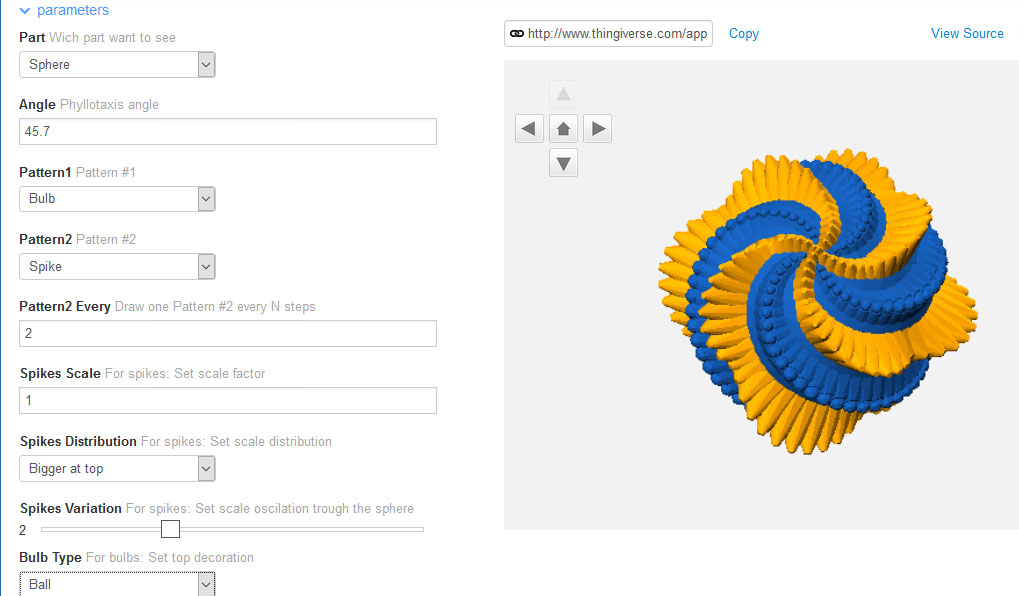
\includegraphics[width=14cm]{Img/WEB/web-maker.jpg}
\centering
\caption{\textbf{ \footnotesize{Interfaz de Customizer con un objeto y sus parametros}}}
\label{fig:customizer}
\end{figure}

\subsection{Beta.Spekle}

Spekle \citep{UCL2018} es un proyecto desarrollado por \textit{The Bartlett School of Architecture UCL}\footnote{\url{https://www.ucl.ac.uk/bartlett/architecture/}} pensado para que los usuarios de Grasshopper puedan compartir diseños paramétricos en la web. 
El proyecto consta de:
\begin{itemize}
    \item Un plugin Spekle, que en combinación con Grasshopper permite establecer los parametros de los modelos y exportarlos a archivos en formato SPK para luego visualizarlos en la web. En la Figura \ref{fig:plugin} se puede ver un ejemplo de uso.
    \item Una aplicación web que permite subir archivos SPK para visualizar los modelos paramétricos con sus respectivas variables, crear versiones modificadas y registrar un historial de los cambios en los modelos. Ver \ref{fig:spekle}
\end{itemize}

\textbf{Beta.Spekle}\footnote{\url{http://beta.speckle.xyz/}} es la versión de desarrollo de la plataforma web y se publica como un proyecto FLOSS que acepta contribuciones de la comunidad.

\begin{figure}[h]
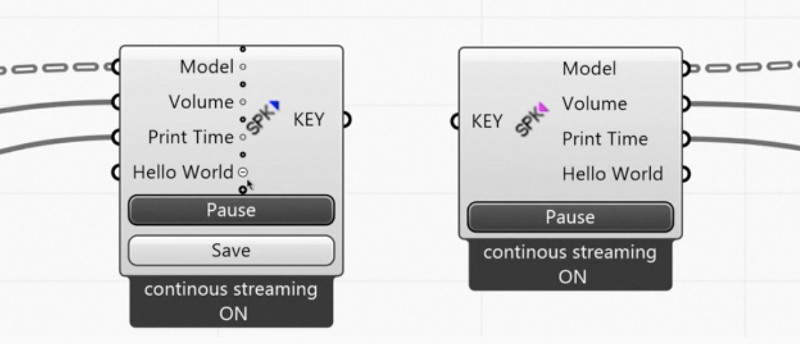
\includegraphics[width=8cm]{Img/WEB/web-plugin.jpg}
\centering
\caption{\textbf{ \footnotesize{Uso de Spekle junto a Grasshopper.}}}
\label{fig:plugin}
\end{figure}

\begin{figure}[h]
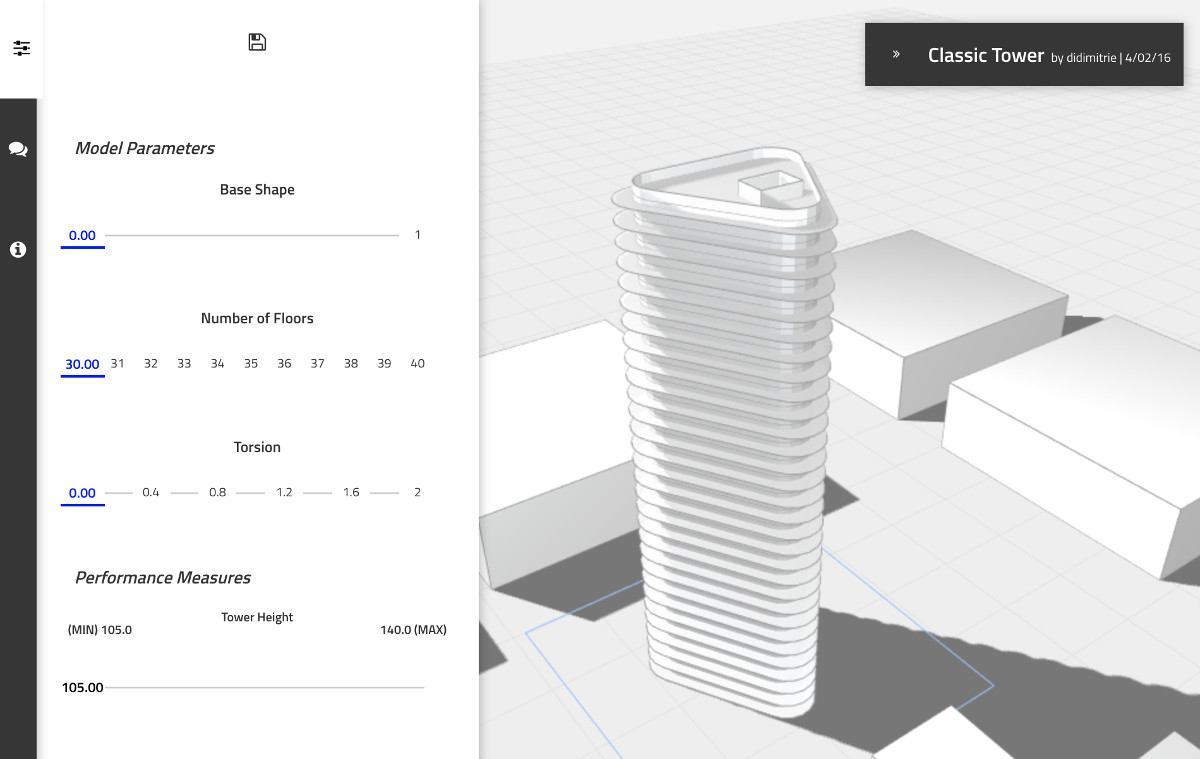
\includegraphics[width=14cm]{Img/WEB/web-spekle.jpg}
\centering
\caption{\textbf{ \footnotesize{Interfaz de beta.spekle, a la izquierda se pueden apreciar los parámetros del modelo.}}}
\label{fig:spekle}
\end{figure}


\subsection{Modelo.io}

Modelo.io\citep{Modelo.io2018} es una plataforma web creada por Qi Su y Tian Deng, orientada a profesionales que trabajan con software CAD como Rhino\footnote{\url{https://www.rhino3d.com/es}} y SketchUp\footnote{\url{https://www.sketchup.com/es}}. Permite una colaboración intuitiva entre los miembros de un equipo para perfeccionar los diseños y presentarlos de forma interactiva.

Mediante modelo, los usuarios visualizan y exploran diseños en 3D, proporcionan comentarios, almacenan archivos de proyectos, se comunican entre los miembros del equipo y puedan crear presentaciones 3D interactivas para los clientes. En la figura \ref{fig:modelo.io} se puede apreciar la vista del modelo y la interacción de los usuarios.

La características más llamativas que incluyen son los recorridos virtuales para arquitectura y la visualización de escenas en realidad virtual.

El servicio ofrece una versión reducida, gratuita para estudiantes registrados. Para acceder a todas las funcionalidades de modelo.io las cuentas son de servicio pago.

\begin{figure}[h]
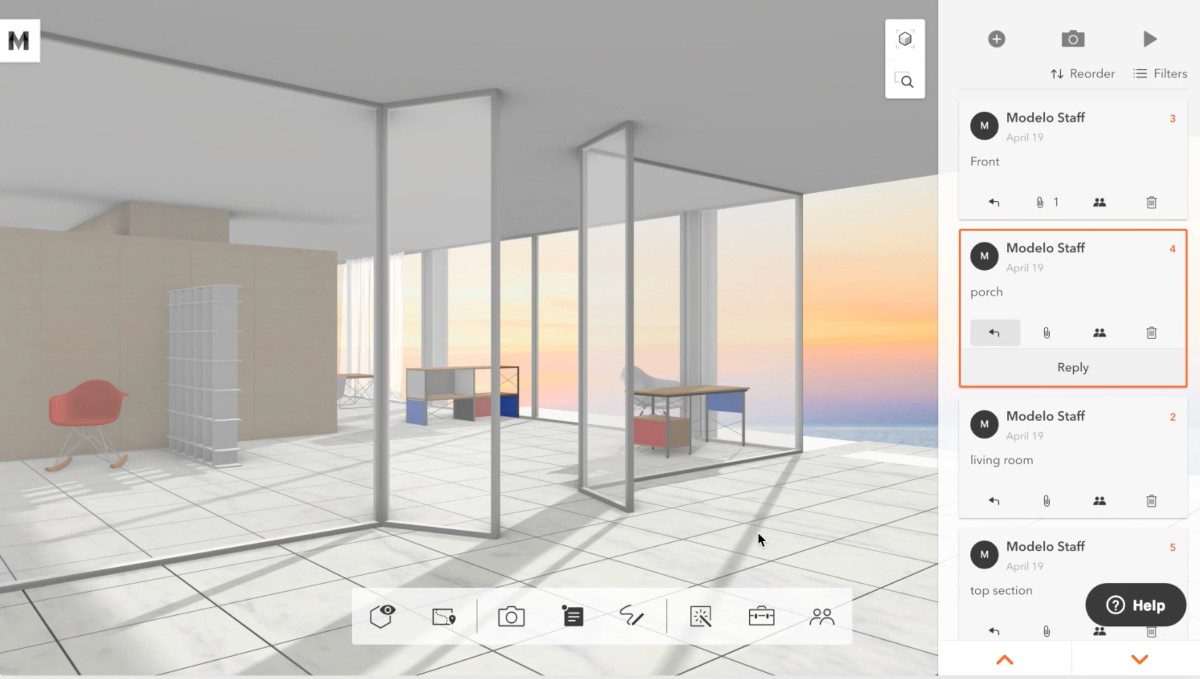
\includegraphics[width=14cm]{Img/WEB/web-modelo.jpg}
\centering
\caption{\textbf{ \footnotesize{Interfaz de Modelo.io, a la derecha se puede apreciar la interacción entre usuarios.}}}
\label{fig:modelo.io}
\end{figure}